% **************************************************************************************************************
% A Classic Thesis Style
% An Homage to The Elements of Typographic Style
%
% Copyright (C) 2015 André Miede http://www.miede.de
%
% If you like the style then I would appreciate a postcard. My address 
% can be found in the file ClassicThesis.pdf. A collection of the 
% postcards I received so far is available online at 
% http://postcards.miede.de
%
% License:
% This program is free software; you can redistribute it and/or modify
% it under the terms of the GNU General Public License as published by
% the Free Software Foundation; either version 2 of the License, or
% (at your option) any later version.
%
% This program is distributed in the hope that it will be useful,
% but WITHOUT ANY WARRANTY; without even the implied warranty of
% MERCHANTABILITY or FITNESS FOR A PARTICULAR PURPOSE.  See the
% GNU General Public License for more details.
%
% You should have received a copy of the GNU General Public License
% along with this program; see the file COPYING.  If not, write to
% the Free Software Foundation, Inc., 59 Temple Place - Suite 330,
% Boston, MA 02111-1307, USA.
%
% **************************************************************************************************************
\RequirePackage{fix-cm} % fix some latex issues see: http://texdoc.net/texmf-dist/doc/latex/base/fixltx2e.pdf
\documentclass[ twoside,openright,titlepage,numbers=noenddot,headinclude,%1headlines,% letterpaper a4paper
                footinclude=true,cleardoublepage=empty,abstractoff, % <--- obsolete, remove (todo)
                BCOR=5mm,paper=a4,fontsize=11pt,%11pt,a4paper,%
                french,american,%
                ]{scrreprt}

%********************************************************************
% Note: Make all your adjustments in here
%*******************************************************
\input{classicthesis-config}
\newcommand{\red}[1]{\textcolor{red}{#1}}
%********************************************************************
\usepackage{enumitem}
\usepackage{amsmath,amssymb,amsfonts}
\usepackage{algorithmic}
\usepackage{graphicx}
\usepackage{csquotes}
\usepackage[inkscapeformat=png]{svg}
\usepackage{textcomp}
\usepackage{xcolor}
\def\BibTeX{{\rm B\kern-.05em{\sc i\kern-.025em b}\kern-.08em
    T\kern-.1667em\lower.7ex\hbox{E}\kern-.125emX}}
\usepackage{amsmath}
\newcommand{\probP}{\text{I\kern-0.15em P}}
% \include{figures/ADTreePreamble}

\usepackage{etoolbox}

% --- Tickz
\usepackage{physics}
\usepackage{amsmath}
\usepackage{tikz}
\usepackage{mathdots}
\usepackage{yhmath}
\usepackage{cancel}
\usepackage{color}
\usepackage{siunitx}
\usepackage{array}
\usepackage{multirow}
\usepackage{amssymb}
\usepackage{gensymb}
\usepackage{tabularx}
\usepackage{extarrows}
\usepackage{booktabs}
\usetikzlibrary{fadings}
\usetikzlibrary{patterns}
\usetikzlibrary{shadows.blur}
\usetikzlibrary{shapes}

\usepackage{tikz}
\usetikzlibrary{shapes.geometric, arrows.meta, positioning}
\usetikzlibrary{positioning, shapes.geometric, arrows.meta, fit}

\tikzstyle{startstop} = [rectangle, rounded corners, minimum width=3cm, minimum height=1cm,text centered, draw=black, fill=gray!10]
\tikzstyle{process} = [rectangle, minimum width=3.5cm, minimum height=1.2cm, text centered, draw=black, fill=blue!10]
\tikzstyle{decision} = [diamond, minimum width=3cm, minimum height=1cm, text centered, draw=black, fill=yellow!20, aspect=2]
\tikzstyle{arrow} = [thick,->,>=stealth]

\usetikzlibrary{decorations.pathreplacing, positioning}


\usepackage{amsmath,amssymb,amsfonts}%
\usepackage{amsthm}%
\usepackage{mathrsfs}%
% \usepackage[title]{appendix}%
% \usepackage{xcolor}%
% \usepackage{textcomp}%
% \usepackage{manyfoot}%
% \usepackage{booktabs}%
% \usepackage{algorithm}%
% \usepackage{algorithmicx}%
% \usepackage{algpseudocode}%
% \usepackage{listings}%

\usepackage{hyperref}

%%%% For camera-ready, use this
%\documentclass[sigconf]{aamas}

\usepackage{listings}
\usepackage{graphicx}
\usepackage{color}
\usepackage{listings}
\usepackage{stfloats}
\usepackage{ragged2e}
% \usepackage[hyphens]{url}
\usepackage{float}
\usepackage[linesnumbered, ruled, vlined]{algorithm2e}


% ---------

\setlength{\extrarowheight}{2.5pt}

\renewcommand{\arraystretch}{0.2}


% \renewcommand{\arraystretch}{1.7}

\newcommand{\before}[1]{\textcolor{red}{#1}}
\newcommand{\after}[1]{\textcolor{green}{#1}}

\newcommand{\old}[1]{\textcolor{orange}{#1}}
\newcommand{\rem}[1]{\textcolor{red}{#1}}
\newcommand{\todo}[1]{\textcolor{orange}{\newline \textit{\textbf{TODO:} #1}} \newline \newline }
%********************************************************************

%********************************************************************
% Bibliographies
%*******************************************************
\addbibresource{references.bib}
\addbibresource[label=ownpubs]{JSoule_publications.bib}
%********************************************************************
% Hyphenation
%*******************************************************
%\hyphenation{put special hyphenation here}

% ********************************************************************
% GO!GO!GO! MOVE IT!
%*******************************************************
\begin{document}
\frenchspacing
\raggedbottom
\selectlanguage{french} % american ngerman
%\renewcommand*{\bibname}{new name}
%\setbibpreamble{}
\pagenumbering{roman}
\pagestyle{plain}
%********************************************************************
% Frontmatter
%*******************************************************
\include{FrontBackmatter/DirtyTitlepage}
\include{FrontBackmatter/Titlepage}
\include{FrontBackmatter/Titleback}

% \cleardoublepage\include{FrontBackmatter/Dedication}
\cleardoublepage%*******************************************************
% Acknowledgments
%*******************************************************
\pdfbookmark[1]{Acknowledgments}{acknowledgments}

% \begin{flushright}{\slshape    
%     We have seen that computer programming is an art, \\ 
%     because it applies accumulated knowledge to the world, \\ 
%     because it requires skill and ingenuity, and especially \\
%     because it produces objects of beauty.} \\ \medskip
%     --- \defcitealias{knuth:1974}{Donald E. Knuth}\citetalias{knuth:1974} \citep{knuth:1974}
% \end{flushright}



\bigskip

\begingroup
\let\clearpage\relax
\let\cleardoublepage\relax
\let\cleardoublepage\relax
\chapter*{Remerciements}

Faire un doctorat peut sembler être un chemin solitaire, mais je ne l’ai certainement pas parcouru seul.

Je tiens tout d’abord à remercier mes directeurs de thèse, Jean-Paul, Michel, Louis-Marie et Paul. Ils m’ont guidé tout au long de ce processus, m’ont permis de découvrir ce qu’est la recherche – y compris les erreurs – mais aussi d’intervenir lorsque c’était nécessaire. Ils ont toujours été là pour moi, même pendant leurs vacances, en prenant le temps de relire mon manuscrit de thèse.

Un grand merci également aux membres de mon jury : X1 et X2, pour leurs relectures, X2 pour avoir assumé le rôle de président du jury et X3 pour avoir révisé mon travail tout au long de mon doctorat.

J’ai rencontré de nombreux étudiants incroyables au cours de mon séjour au laboratoire. Je voudrais surtout mentionner Arthur, Vincent, Thinh et Karem pour m’avoir accueilli. Je tiens à remercier Minh Tuan, Sébastien et Maximilian pour leur gentillesse et pour tous les échanges que nous avons eu.

Je remercie également François Suro et Simon Gay, qui m’ont donné régulièrement des retours et m’ont permis de garder le cap quand j’étais motivée mais manquais encore de confiance en mon travail.

Un grand merci à Clément Raïevsky, Romain Liévin et Oum-el-Kheir Aktouf pour m’avoir aidé dans mes premières expériences d’enseignement. Travailler au LCIS n’aurait pas été aussi facile sans Patricia et Carole qui m'ont aidé pour affronter la montagne de formalités administratives, ainsi qu'Arthur et Marie qui m'ont permis d'utiliser les moyens techniques dont j'avais besoin.

Je tiens également à remercier mes amis Dorian et ThoSMA, qui sont également sur ce chemin du doctorat, ainsi que Joaquin, qui a toujours été là pour m’aider à faire une pause dans mes réflexions sur mes études.

Et enfin, je dois tout à ma famille, qui m’a soutenue sans réserve tout au long de ma vie. Rien de tout cela n’aurait été possible sans eux.


\endgroup




%\cleardoublepage\include{FrontBackmatter/Foreword}
\cleardoublepage
%*******************************************************
% Abstract
%*******************************************************
%\renewcommand{\abstractname}{Abstract}
\pdfbookmark[1]{Abstract}{Abstract}
\begingroup
\let\clearpage\relax
\let\cleardoublepage\relax
\let\cleardoublepage\relax

\begin{otherlanguage}{ngerman}
    \pdfbookmark[1]{Zusammenfassung}{Zusammenfassung}
    \chapter*{Résumé}
    Kurze Zusammenfassung des Inhaltes in deutscher Sprache\dots

    \medskip

    \

    \noindent MOTS-CLEFS :
    Système Multi-Agent \raisebox{0.25ex}{\tiny$\bullet$} Cyberdéfense \raisebox{0.25ex}{\tiny$\bullet$} Apprentissage 
    
    \hskip6em\relax par Reinforcement Multi-Agent

\end{otherlanguage}


\vfill

\chapter*{Abstract}
Short summary of the contents in English\dots a great guide by
Kent Beck how to write good abstracts can be found here:

\medskip

\

\noindent KEYWORDS :
Multi-Agent Systems \raisebox{0.25ex}{\tiny$\bullet$} Cyberdefense \raisebox{0.25ex}{\tiny$\bullet$} Multi-Agent 

\hskip5.7em\relax Reinforcement Learning

\endgroup

\vfill
\cleardoublepage %*******************************************************
% Publications
%*******************************************************
\pdfbookmark[1]{Publications}{publications}
\chapter*{Publications}

%\noindent Put your publications from the thesis here. The packages \texttt{multibib} or \texttt{bibtopic} etc. can be used to handle multiple different bibliographies in your document.

\begin{refsection}[ownpubs]

    \noindent JOURNAUX
    \small
    \nocite{soulej2025jaamas}

    \printbibliography[keyword=journal, heading=none]

    \

    \noindent CONFERENCES INTERNATIONALES
    \small
    \nocite{soule2024moise_marl}
    \nocite{soule2024marl}
    \nocite{soulej2023sim}
    \nocite{soulej2025cloud}
    \printbibliography[keyword=international, heading=none]

    \

    \noindent CONFERENCES NATIONALES
    \nocite{soule2023jfsmathese}
    \nocite{soule2023ressithese}
    \nocite{soule2023rjciathese}
    \nocite{soule2024outil}
    \nocite{soule2024approche}
    \nocite{soule2025jfsma}
    \printbibliography[keyword=national, heading=none]

\end{refsection}

\pagestyle{scrheadings}
\cleardoublepage %*******************************************************
% Table of Contents
%*******************************************************
%\phantomsection
\refstepcounter{dummy}
\pdfbookmark[1]{\contentsname}{tableofcontents}
\setcounter{tocdepth}{2} % <-- 2 includes up to subsections in the ToC
\setcounter{secnumdepth}{3} % <-- 3 numbers up to subsubsections
\manualmark
\markboth{\spacedlowsmallcaps{\contentsname}}{\spacedlowsmallcaps{\contentsname}}
\tableofcontents
\automark[section]{chapter}
\renewcommand{\chaptermark}[1]{\markboth{\spacedlowsmallcaps{#1}}{\spacedlowsmallcaps{#1}}}
\renewcommand{\sectionmark}[1]{\markright{\thesection\enspace\spacedlowsmallcaps{#1}}}
%*******************************************************
% List of Figures and of the Tables
%*******************************************************
\clearpage

\begingroup
\let\clearpage\relax
\let\cleardoublepage\relax
\let\cleardoublepage\relax
%*******************************************************
% List of Figures
%*******************************************************    
%\phantomsection 
\refstepcounter{dummy}
% \addcontentsline{toc}{chapter}{\listfigurename}
\pdfbookmark[1]{\listfigurename}{lof}
\listoffigures

\pagebreak

%*******************************************************
% List of Tables
%*******************************************************
%\phantomsection 
\refstepcounter{dummy}
% \addcontentsline{toc}{chapter}{\listtablename}
\pdfbookmark[1]{\listtablename}{lot}
\listoftables

\pagebreak

%*******************************************************
% List of Listings
%*******************************************************      
%\phantomsection 
% \refstepcounter{dummy}
% % \addcontentsline{toc}{chapter}{\lstlistlistingname}
% \pdfbookmark[1]{List de Listings}{lol}
% \lstlistoflistings

% \pagebreak

%*******************************************************
% Acronyms
%*******************************************************
%\phantomsection 
\refstepcounter{dummy}
% \addcontentsline{toc}{chapter}{Liste d'acronymes}
\pdfbookmark[1]{Liste d'acronymes}{acronyms}
\markboth{\spacedlowsmallcaps{Liste d'acronymes}}{\spacedlowsmallcaps{Liste d'acronymes}}
\chapter*{Liste d'acronymes}
\begin{acronym}[UMLX]
  \acro{ACD}{\textit{Automated Cyber Defense}}
  \acro{ACO}{\textit{Autonomous Cyber Operation}}
  \acro{AD}{\textit{Attack-Defense}}
  \acro{AEC}{\textit{Agent Environment Cycle}}
  \acro{AGR}{\textit{Agents, Groups, Roles}}
  \acro{AHPA}{\textit{Advanced Horizontal Pod Autoscaler}}
  \acro{AICA}{\textit{Autonomous Intelligent Cyberdefense Agent}}
  \acro{AMD}{\textit{Advanced Micro Devices}}
  \acro{ANL-AUT}{\textit{Automated Analysis}}
  \acro{ANL-MAN}{\textit{Manual Analysis}}
  \acro{ANSSI}{Agence Nationale de la Sécurité des Systèmes d'Information}
  \acro{AOSE}{\textit{Agent Oriented Software Engineering}}
  \acro{API}{\textit{Application Programming Interface}}
  \acro{APT}{\textit{Advanced Persistent Threat}}
  \acro{ASAP}{\textit{As Soon As Possible}}
  \acro{Auto-TEMM}{\textit{Automatic Trajectory-based Evaluation in MOISE+MARL}}
  \acro{AutoPentest-DRL}{\textit{Automated Penetration Testing Using Deep Reinforcement Learning}}
  \acro{AWARE}{\textit{Adaptive Web-based Analysis for REsilience}}
  \acro{BDI}{\textit{Belief-Desire-Intention}}
  \acro{C2}{\textit{Command and Control}}
  \acro{CAGE}{\textit{Cyber Automated Game-based Evaluation}}
  \acro{CANDLES}{\textit{Cybersecurity ANomaly Detection via Learning and Evaluation System}}
  \acro{CAV}{\textit{Concept Activation Vector}}
  \acro{CIA}{\textit{Confidentiality, Integrity, and Availability}}
  \acro{CLAP}{\textit{Contrastive Language-Audio Pretraining}}
  \acro{CLI}{\textit{Command Line Interface}}
  \acro{CLS}{\textit{Classification token}}
  \acro{CMDP}{\textit{Constrained Markov Decision Process}}
  \acro{COMA}{\textit{Counterfactual Multi-Agent Policy Gradients}}
  \acro{COPA}{\textit{Combined Autoscaling for Kubernetes}}
  \acro{CPO}{\textit{Constrained Policy Optimization}}
  \acro{CPU}{\textit{Central Processing Unit}}
  \acro{CSIRT}{\textit{Computer Security Incident Response Team}}
  \acro{CSLE}{\textit{Cyber Security Learning Environment}}
  \acro{CTDE}{\textit{Centralized Training Decentralized Execution}}
  \acro{CTF}{\textit{Capture The Flag}}
  \acro{CUDA}{\textit{Compute Unified Device Architecture}}
  \acro{CyberBattleSim}{\textit{Cyber Battle Simulator}}
  \acro{CyberVAN}{Cyber Virtual Ad-hoc Networking}
  \acro{CybMASDE}{\textit{Cyberdefense Multi-Agent System Development Environment}}
  \acro{CybORG}{\textit{Cyber Operations Research Gym}}
  \acro{CYST}{\textit{Cyber Security Simulation Testbed}}
  \acro{DARPA}{\textit{Defense Advanced Research Projects Agency}}
  \acro{DB}{\textit{Database}}
  \acro{DCOP}{\textit{Distributed Constraint Optimization Problem}}
  \acro{DCQL}{\textit{Deep Constrained Q-Learning}}
  \acro{DDS}{\textit{Data Distribution Service}}
  \acro{Dec-MDP}{\textit{{Decentralized Markov Decision Processes}}}
  \acro{Dec-POMDP}{\textit{Decentralized Partially Observable Markov Decision Process}}
  \acro{DETERLab}{cyber DEfense Technology Experimental Research Laboratory}
  \acro{DQN}{\textit{Deep Q-Network}}
  \acro{DRL}{\textit{Deep Reinforcement Learning}}
  \acro{DS}{\textit{Deontic Specifications}}
  \acro{DTW}{\textit{Dynamic Time Wrapping}}
  \acro{EmuLab}{\textit{Emulation Laboratory}}
  \acro{ES}{\textit{Email Server}}
  \acro{FN}{Faux Négatif}
  \acro{FOF}{\textit{Functional Organizational Fit}}
  \acro{FP}{Faux Positif}
  \acro{FS}{\textit{Functional Specifications}}
  \acro{FW}{\textit{Firewall}}
  \acro{GARD}{\textit{Guaranteed AI Robustness against Deception}}
  \acro{GPU}{\textit{Graphics Processing Unit}}
  \acro{GR}{\textit{Graphes de Raisonnement}}
  \acro{HPA}{\textit{Horizontal Pod Autoscaler}}
  \acro{HPC}{\textit{High Performance Computing}}
  \acro{HPO}{\textit{Hyper-Parameter Optimization}}
  \acro{HRL}{\textit{Hierarchical Reinforcement Learning}}
  \acro{IA}{Intelligence Artificielle}
  \acro{IAM}{\textit{Identity and Access Manager}}
  \acro{ID}{\textit{Intrusion Detection}}
  \acro{IDS}{\textit{Intrusion Detection System}}
  \acro{IoC}{\textit{Indicator of Compromission}}
  \acro{IOC}{\textit{Indicator of Compromise}}
  \acro{IP}{\textit{Internet Protocol}}
  \acro{IQL}{\textit{Independent Q-Learning}}
  \acro{JAX}{\textit{Just-in-time Accelerated computation (Google)}}
  \acro{JOPM}{\textit{Joint-Observation Prediction Model}}
  \acro{JSON}{\textit{JavaScript Object Notation}}
  \acro{KARMA}{\textit{Kubernetes Autoscaling with Resilient Multi-Agent system}}
  \acro{KL}{\textit{Kullback–Leibler divergence}}
  \acro{KNN}{\textit{K-Nearest Neighbors}}
  \acro{KOSMOS}{\textit{Kubernetes Vertical and Horizontal Resource Autoscaling}}
  \acro{LCS}{\textit{Longest Common Sequence}}
  \acro{LGPL}{\textit{GNU Lesser General Public License}}
  \acro{LIME}{\textit{Local Interpretable Model-agnostic Explanations}}
  \acro{LLM}{\textit{Large Language Model}}
  \acro{LM}{\textit{Language Model}}
  \acro{LR}{\textit{Learning Rate}}
  \acro{LRP}{\textit{Layer-wise Relevance Propagation}}
  \acro{LSTM}{\textit{Long-Short Term Memory}}
  \acro{MADDPG}{\textit{Multi-Agent Deep Deterministic Policy Gradient}}
  \acro{MAE}{\textit{Mean Absolute Error}}
  \acro{MAMAD}{\textit{MOISE+MARL Assisted MAS Design}}
  \acro{MAPPO}{\textit{Multi-Agent Proximal Policy Optimization}}
  \acro{MARL}{\textit{Multi-Agent Reinforcement Learning}}
  \acro{MARLlib}{\textit{Multi-Agent Reinforcement Learning Library}}
  \acro{MAS}{\textit{Multi-Agent System}}
  \acro{MASCARA}{\textit{Multi-Agent System Centric AICA Reference Architecture}}
  \acro{MAVIPER}{\textit{Multi-Agent VIrtual PERimeter}}
  \acro{MAWM}{\textit{Multi-Agent World Models}}
  \acro{MBRL}{\textit{Model-based Reinforcement Learning}}
  \acro{MCAS}{\textit{Multi-Cyberdefense Agent Simulator}}
  \acro{MDP}{\textit{Markov Decision Process}}
  \acro{MEM}{\textit{Memory}}
  \acro{MENTOR}{\textit{Multi-agent Environment for Networked Training, Operations and Response}}
  \acro{MIT}{\textit{Massachusetts Institute of Technology}}
  \acro{ML}{\textit{Machine Learning}}
  \acro{MLP}{\textit{Multi-Layer Perceptron}}
  \acro{MMA}{\textit{MOISE+MARL API}}
  \acro{MMD}{\textit{Maximum Mean Discrepancy}}
  \acro{MOD-AUT}{\textit{Automated Modelling}}
  \acro{MOD-MAN}{\textit{Manual Modelling}}
  \acro{MSE}{\textit{Mean Squared Error}}
  \acro{MTA}{Modéliser-Entraîner-Analyser}
  \acro{NASim}{Network Attack Simulator}
  \acro{NASimEmu}{\textit{Network Attack Simulator \& Emulator}}
  \acro{NIST}{\textit{National Institute of Standards and Technology}}
  \acro{NVIDIA}{\textit{NVIDIA Corporation}}
  \acro{ODec-POMDP}{\textit{Observation-based Dec-POMDP}}
  \acro{OF}{\textit{Organizational Fit}}
  \acro{OPM}{\textit{Observation Prediction Model}}
  \acro{OS}{\textit{Organizational Specifications}}
  \acro{OTAN}{Organisation du Traité de l'Atlantique Nord}
  \acro{PAM}{\textit{Privileged Access Management}}
  \acro{PCA}{\textit{Principal Component Analysis}}
  \acro{PenGym}{\textit{Penetration Testing Gym}}
  \acro{PILCO}{\textit{Probabilistic Inference for Learning Control}}
  \acro{POMDP}{\textit{Partially Observable Markov Decision Process}}
  \acro{POSG}{\textit{Partially Observable Stochastic Games}}
  \acro{PPO}{\textit{Proximal Policy Optimization}}
  \acro{PS}{\textit{Privileged Service}}
  \acro{PSSI}{Politique de sécurité du système d'information}
  \acro{QMix}{\textit{Monotonic Value Function Factorization for Deep Multi-Agent Reinforcement Learning}}
  \acro{QMIX}{\textit{Monotonic Value Function Factorisation for Deep Multi-Agent Reinforcement Learning}}
  \acro{RAM}{\textit{Random Access Memory}}
  \acro{REST}{\textit{Representational State Transfer}}
  \acro{RG}{\textit{Règles Génératives}}
  \acro{RL}{\textit{Reinforcement Learning}}
  \acro{RLDM}{\textit{Recurrent Latent Dynamics Model}}
  \acro{RNN}{\textit{Recurrent Neural Network}}
  \acro{ROMA}{\textit{Role-Oriented Multi-Agent Reinforcement Learning}}
  \acro{ROS}{\textit{Robot Operating System}}
  \acro{SCYTHE}{\textit{SCYTHE Cybersecurity Platform}}
  \acro{SDN}{\textit{Software Defined Networking}}
  \acro{SHAP}{\textit{SHapley Additive exPlanations}}
  \acro{SMA}{Système Multi-Agent}
  \acro{SOC}{\textit{Security Operation Center}}
  \acro{SOF}{\textit{Structural Organizational Fit}}
  \acro{SP}{Séquence Parente}
  \acro{SPOF}{\textit{Single Point Of Failure}}
  \acro{SS}{\textit{Security Service}}
  \acro{SSM}{\textit{Structural Specifications}}
  \acro{SVM}{\textit{Support Vector Machine}}
  \acro{TAB}{\textit{Terminal Access Broker}}
  \acro{TEMM}{\textit{Trajectory-based Evaluation in MOISE+MARL}}
  \acro{TP}{\textit{Trajectory-based Pattern}}
  \acro{TPE}{\textit{Tree-structured Parzen Estimator}}
  \acro{TRF-AUT}{\textit{Automated Transferring}}
  \acro{TRF-MAN}{\textit{Manual Transferring}}
  \acro{TRN-CON}{\textit{Constrained/Guided Training}}
  \acro{TRN-UNC}{\textit{Unconstrained Training}}
  \acro{TRPO}{\textit{Trust Region Policy Optimization}}
  \acro{TTP}{Tactiques, Techniques et Procédures}
  \acro{UX}{\textit{User eXperience}}
  \acro{VAE}{\textit{Variational Auto Encoder}}
  \acro{VDN}{\textit{Value-Decomposition Networks}}
  \acro{VM}{\textit{Virtual Machine}}
  \acro{VPN}{\textit{Virtual Private Network}}
  \acro{WS}{\textit{Web Server}}
  \acro{XAI}{\textit{eXplainable Artificial Intelligence}}

\end{acronym}
\acrodefplural{SMA}[SMA]{Systèmes Multi-Agents}
\endgroup

\pagebreak


%********************************************************************
% Mainmatter
%*******************************************************
\cleardoublepage\pagenumbering{arabic}
\cleardoublepage


\part{Introduction générale et construction de la démarche de recherche}

\chapter{Contexte, concepts et problématique générale}
% Objectif : poser les fondations du domaine de recherche, identifier les enjeux de la cyberdéfense moderne, et formuler la question centrale de la thèse.

\section{Définitions, concepts et panorama de la recherche en Cyberdéfense}\label{sec:cyberdef-panorama}

% L'objectif de cette section est de donner un aperçu général du domaine de la Cyberdéfense.
% - TODO : Définitions consensuelles, concepts consensuelles, but/objectifs consensuels du domaine, faire un aperçu du panorama des différents axes des travaux du domaine (quel sont les sujets actuels), expliquer dans quel partie du domaine nous comptons contribuer.
% - TODO : Il faut mentionner que l'idée d'une Cyberdéfense décentralisée et distribuée comme dans un SMA de Cyberdéfense est quasi absent de la littérature

\section{Définitions, concepts et panorama de la recherche en Cyberdéfense}

La cyberdéfense est aujourd'hui au cœur des préoccupations stratégiques des États, des entreprises critiques et des alliances internationales. Alors que les cyberattaques se complexifient, se distribuent et s'industrialisent, la réponse défensive nécessite non seulement des mécanismes techniques avancés, mais aussi une approche systémique intégrant des considérations organisationnelles, cognitives et dynamiques \cite{rudner2020state, nicolas2021souverainete, ota2019cybersecurity}. Cette section vise à établir un socle conceptuel sur la cyberdéfense en posant des définitions fondamentales, en identifiant les principales dimensions du domaine et en esquissant les tendances de recherche actuelles.

\subsection*{Définition de la cyberdéfense}

Le terme « cyberdéfense » recouvre un spectre de pratiques qui dépassent la cybersécurité technique au sens strict. Selon l'OTAN, elle englobe « la protection et la défense des systèmes d'information et de communication militaires contre les cybermenaces, y compris par des capacités actives de réponse » \cite{nato-cyberdefense}. Cette définition dépasse donc la simple prévention pour inclure la détection, la réaction et l'adaptation dans un contexte opérationnel.

En France, l'Agence nationale de la sécurité des systèmes d'information (ANSSI) distingue la cybersécurité comme la « sécurité des systèmes d'information », tandis que la cyberdéfense est associée à des capacités militaires ou souveraines impliquant une posture active, voire offensive, de réponse aux menaces \cite{anssi2015guide}. Cette distinction est illustrée dans la \textbf{Figure~\ref{fig:cyberdefense-vs-cybersecurite}}, qui met en parallèle les périmètres conceptuels des deux approches.

\begin{figure}[H]
    \centering
    \fbox{\begin{minipage}{0.9\textwidth}
            \vspace{3cm}
            \centering
            \textit{Schéma comparatif des périmètres conceptuels entre cybersécurité (protection, prévention) et cyberdéfense (détection, réaction, contre-mesures, adaptation)}.
            \vspace{3cm}
        \end{minipage}}
    \caption{Distinction conceptuelle entre cybersécurité et cyberdéfense}
    \label{fig:cyberdefense-vs-cybersecurite}
\end{figure}

\subsection*{Composantes fondamentales de la cyberdéfense}

Les systèmes de cyberdéfense modernes peuvent être analysés selon plusieurs dimensions clés :

\begin{itemize}
    \item \textbf{La détection des menaces}, incluant la surveillance, l'analyse d'anomalies et les systèmes de détection d'intrusion (IDS), souvent fondés sur des approches statistiques ou d'apprentissage automatique \cite{sommer2010outside}.

    \item \textbf{La réaction aux incidents}, allant de la neutralisation locale à la réponse coordonnée multi-niveaux (CSIRT, SOC, etc.) \cite{parsons2016managing}.

    \item \textbf{L'automatisation et la prise de décision}, avec l'émergence de systèmes intelligents cherchant à réduire la dépendance aux opérateurs humains \cite{kim2018survey, wood2018taxonomy}.

    \item \textbf{La résilience}, qui implique non seulement le rétablissement du service, mais aussi l'apprentissage adaptatif face aux attaques futures \cite{kozlowski2013emergence, cashell2004cyber}.
\end{itemize}

Ces éléments ne sont pas indépendants, mais interagissent dans une boucle complexe d'observation, d'analyse, de décision et d'action, parfois appelée boucle OODA (Observe, Orient, Decide, Act), empruntée aux modèles décisionnels militaires.

\subsection*{Acteurs, échelles et hybridité des systèmes de défense}

L'un des traits distinctifs de la cyberdéfense moderne est son caractère multi-échelle. Les dispositifs de défense peuvent être individuels (terminaux, honeypots), organisationnels (réseaux d'entreprise, datacenters) ou systémiques (infrastructures critiques, réseaux souverains). Ces niveaux interagissent selon une logique hiérarchique ou coopérative, comme illustré en \textbf{Figure~\ref{fig:ecologie-defense}}, qui propose une vision écosystémique des dispositifs de cyberdéfense.

\begin{figure}[H]
    \centering
    \fbox{\begin{minipage}{0.9\textwidth}
            \vspace{3cm}
            \centering
            \textit{Schéma illustrant les différentes échelles de la cyberdéfense : du terminal isolé jusqu'aux structures de défense nationale, en passant par les centres de coordination et les dispositifs d'orchestration automatisée.}
            \vspace{3cm}
        \end{minipage}}
    \caption{Écologie des systèmes de cyberdéfense distribuée}
    \label{fig:ecologie-defense}
\end{figure}

De plus, l'essor de l'intelligence artificielle a conduit à l'hybridation croissante des systèmes de cyberdéfense : les capacités humaines sont de plus en plus soutenues par des agents logiciels, parfois autonomes, agissant à la place ou en complément des analystes. Ces agents s'intègrent dans ce que l'OTAN appelle les AICA (Autonomous Intelligent Cyber Agents), qui seront développés plus avant dans la suite du chapitre.

\subsection*{Tendances de recherche et enjeux contemporains}

Les travaux de recherche en cyberdéfense se structurent actuellement autour de plusieurs axes clés :

\begin{itemize}
    \item \textbf{L'application de l'apprentissage machine (ML)} pour la détection d'attaques, le renforcement de la résilience ou la génération de réponses \cite{hammar2021autonomous, mitrokotsa2018machine}.

    \item \textbf{Les environnements de simulation pour la formation, l'évaluation et la mise à l'échelle des stratégies de défense}, comme les bancs d'essai CybORG \cite{cyborg2021} ou Yawning Titan \cite{yawning2022}.

    \item \textbf{L'intégration de cadres organisationnels et cognitifs} pour améliorer la coordination et l'explicabilité des agents de défense \cite{ferber1997multi, moise2002}.

    \item \textbf{La recherche d'architectures décentralisées et autonomes}, répondant à l'émergence d'attaques de plus en plus distribuées et adaptatives \cite{asap2022}.
\end{itemize}

Enfin, un enjeu transversal majeur réside dans la \textit{confiance} : comment garantir que les décisions prises par des systèmes autonomes soient justes, explicables, sûres et alignées avec les objectifs stratégiques ? C'est cette interrogation qui conduit progressivement la recherche à s'intéresser à des modèles hybrides, mariant \textit{auto-organisation}, \textit{rôles organisationnels} et \textit{apprentissage}.

\begin{figure}[H]
    \centering
    \fbox{\begin{minipage}{0.9\textwidth}
            \vspace{3cm}
            \centering
            \textit{Illustration des courants de recherche en cyberdéfense avec leurs principaux enjeux techniques, scientifiques et sociétaux.}
            \vspace{3cm}
        \end{minipage}}
    \caption{Panorama des axes de recherche en cyberdéfense}
    \label{fig:panorama-cyberdefense}
\end{figure}

\vspace{0.3cm}
Ainsi, la cyberdéfense moderne dépasse largement le cadre de la simple sécurité informatique. Elle implique une compréhension intégrée des dynamiques adverses, des structures de coordination et des capacités adaptatives d'un système défensif désormais distribué, intelligent, et potentiellement autonome.


\section{Évolution des menaces, défis et besoins en cyberdéfense autonome et émérgence d'une approche distribuée et décentralisée de la Cyberdéfense}\label{sec:evolution-menaces}

% L'objectif de cette section est de montrer que les nouvelles menaces, défis liés aux attaques décentralisées et distribuées (autonomes car aidées des nouvelles prouesses de l'IA qui les rendent très réactifs) font apparaitre de nouveaux défis qui sont prises en compte dans la littérature principalement par les AICA et par d'autres travaux dans une moindre mesure.
% Cette section doit donc faire la transition entre une approche mono-agent de la Cyberdéfense et une approche multi-agent mais sans rentrer dans le détail théorique du domaine des SMAs (car c'est l'objet de la section suivante).

\subsection*{L'évolution des menaces : vers des attaques plus autonomes et distribuées}

Au fil des dernières décennies, les cyberattaques ont évolué de simples actions opportunistes vers des opérations organisées, massives, souvent coordonnées par des entités disposant de ressources considérables. Aujourd'hui, de nombreuses attaques présentent un haut degré d'automatisation et d'adaptabilité.

Par exemple, les malwares modernes intègrent des capacités :
\begin{itemize}
    \item d'\textbf{auto-propagation} à travers des réseaux distribués ;
    \item de \textbf{détection d'environnement} pour contourner les honeypots ou systèmes de sandboxing ;
    \item de \textbf{mutation de code} (polymorphisme) pour échapper aux signatures ;
    \item de \textbf{commandement décentralisé} (via DHT ou blockchain) pour éviter les points de défaillance uniques.
\end{itemize}

\begin{figure}[H]
    \centering
    \fbox{
        \begin{minipage}[c][4cm][c]{0.9\linewidth}
            \centering
            \textit{Illustration à insérer : Chronologie des évolutions des cybermenaces (2000–2025), mettant en évidence l'augmentation de l'autonomie, de la distribution et de la coordination des attaques.}
        \end{minipage}
    }
    \caption{Évolution temporelle des menaces cybernétiques}
    \label{fig:evolution-menaces}
\end{figure}

Cette montée en complexité place les capacités défensives traditionnelles — souvent statiques et centralisées — dans une position de faiblesse. L'environnement dans lequel opèrent les systèmes d'information est devenu dynamique, hostile, et en constante mutation.

\vspace{0.5em}
\subsection*{Les limites des approches défensives traditionnelles}

Les systèmes de défense classiques reposent souvent sur :
\begin{itemize}
    \item des bases de règles statiques (signatures, seuils) ;
    \item une infrastructure hiérarchisée avec des nœuds centraux de décision ;
    \item des flux d'informations remontant vers un SOC (Security Operation Center) pour analyse humaine.
\end{itemize}

Dans des contextes critiques comme les environnements militaires, industriels ou embarqués, ces approches se heurtent à plusieurs limites :
\begin{itemize}
    \item \textbf{latence décisionnelle trop élevée} face à des attaques rapides ;
    \item \textbf{fragilité face aux attaques DDoS ou de coupure de communication} centralisée ;
    \item \textbf{difficulté de couverture dynamique} d'environnements distribués hétérogènes ;
    \item \textbf{charge cognitive importante} sur les opérateurs humains.
\end{itemize}

Ces limites soulignent la nécessité de repenser l'architecture défensive non plus comme un centre décisionnel unique, mais comme un \textbf{système multi-agent auto-adaptatif}.

\vspace{0.5em}
\subsection*{Vers une cyberdéfense autonome et distribuée}

Pour répondre à ces défis, plusieurs initiatives récentes ont émergé, notamment sous l'impulsion de programmes militaires ou industriels de nouvelle génération. L'une des plus notables est le concept d'\textbf{agent AICA} (Autonomous Intelligent Cyber Agent), proposé dans le cadre de travaux de l'OTAN et de la DARPA.

Un agent AICA est un module logiciel embarqué ou distribué, disposant de capacités autonomes pour :
\begin{itemize}
    \item \textbf{observer} son environnement local,
    \item \textbf{prendre des décisions défensives},
    \item \textbf{coordonner avec d'autres agents},
    \item et \textbf{agir rapidement et localement}.
\end{itemize}

\begin{figure}[H]
    \centering
    \fbox{
        \begin{minipage}[c][4.2cm][c]{0.9\linewidth}
            \centering
            \textit{Illustration à insérer : Schéma d'un système AICA multi-agent déployé sur un réseau, montrant les interactions entre agents et les actions locales.}
        \end{minipage}
    }
    \caption{Principe d'un système AICA distribué}
    \label{fig:aica-system}
\end{figure}

Ce modèle vise à réduire les délais de réponse, à assurer une couverture continue et à s'adapter dynamiquement à l'évolution des menaces. Il implique cependant plusieurs problématiques : comment concevoir un tel système ? comment coordonner les agents ? comment garantir leur sûreté de fonctionnement ?

\vspace{0.5em}
\subsection*{Justification d'une approche multi-agent et organisée}

Une approche multi-agent décentralisée permettrait de :
\begin{itemize}
    \item \textbf{scaler horizontalement} la défense sur des infrastructures complexes (cloud, edge, systèmes embarqués) ;
    \item \textbf{réagir localement} sans dépendre d'un nœud central ;
    \item \textbf{s'auto-organiser en cas de panne ou d'attaque} sur certaines zones du système.
\end{itemize}

Cependant, pour être efficace, cette approche doit dépasser la simple distribution et intégrer une \textbf{organisation explicite} entre les agents, définissant leurs rôles, leurs interactions, et les objectifs collectifs qu'ils poursuivent.

C'est précisément ce manque qui est au cœur de la problématique de cette thèse : concevoir un \textbf{Système Multi-Agent de Cyberdéfense auto-organisé}, guidé par une organisation explicite et capable de s'adapter en continu à des environnements instables et potentiellement hostiles.

\begin{figure}[H]
    \centering
    \fbox{
        \begin{minipage}[c][4cm][c]{0.9\linewidth}
            \centering
            \textit{Illustration à insérer : Comparatif entre un SMA non-organisé (agents isolés) et un SMA organisé (agents avec rôles, objectifs, coordination explicite)}
        \end{minipage}
    }
    \caption{De la distribution à l'organisation explicite dans les SMA de cyberdéfense}
    \label{fig:orga-sma-cyber}
\end{figure}

Cette intuition sera développée dans les sections suivantes à travers l'analyse du domaine des Systèmes Multi-Agents, de leurs modèles organisationnels, et la formalisation progressive de notre problématique de recherche.



\section{Définitions, concepts et panorama de la recherche sur les SMA}\label{sec:sma-concepts}

% L'objectif de cette section est de donner les définitions consensuelles, concepts consensuels (auto-organisation, re-organisation...), buts/objectifs consensuels du domaine, faire un aperçu du panorama des différents axes des travaux du domaine (quel sont les sujets actuels), expliquer dans quel partie du domaine nous comptons contribuer.
% Il s'agit, dans cette section, de faire suite à la section précédente qui introduit l'idée de l'approche multi-agent pour la Cyberdéfense. Cette section, doit donc renseigner le lecteur sur tout ce qu'il doit savoir sur le domaine des SMAs.

\subsection*{Pourquoi s'intéresser aux Systèmes Multi-Agents ?}

Les Systèmes Multi-Agents (SMA) constituent une approche paradigmatique de modélisation et de résolution de problèmes distribués. Un SMA est défini comme un ensemble d'agents autonomes interagissant dans un environnement commun, souvent partiellement observable, dans le but d'accomplir des tâches localement ou collectivement.

Ces agents sont capables :
\begin{itemize}
    \item de percevoir leur environnement (par des capteurs logiciels ou physiques),
    \item de prendre des décisions de manière autonome (en suivant une politique locale ou une coordination globale),
    \item d'interagir avec d'autres agents (coopération, compétition, négociation, etc.).
\end{itemize}

\begin{figure}[H]
    \centering
    \fbox{
        \begin{minipage}[c][4cm][c]{0.9\linewidth}
            \centering
            \textit{Illustration à insérer : Schéma générique d'un SMA montrant des agents, leurs observations locales, leurs décisions et les interactions (messages, coordination, etc.).}
        \end{minipage}
    }
    \caption{Représentation générale d'un Système Multi-Agent}
    \label{fig:sma-schema}
\end{figure}

Dans un contexte comme la cyberdéfense, les SMA présentent un intérêt particulier : ils permettent de distribuer les capacités de détection, d'analyse et de réponse sur différents nœuds du réseau, tout en autorisant des mécanismes de coopération, de redondance et de reconfiguration.

\vspace{0.5em}
\subsection*{Concepts fondamentaux : autonomie, organisation et adaptabilité}

Un SMA ne se réduit pas à une simple juxtaposition d'agents. Plusieurs concepts clés caractérisent ce paradigme :

\begin{itemize}
    \item \textbf{Autonomie} : chaque agent peut percevoir, raisonner et agir sans supervision directe ;
    \item \textbf{Interaction} : les agents peuvent échanger des informations, coordonner leurs actions ou négocier ;
    \item \textbf{Organisation} : les agents peuvent être structurés dans des rôles, missions, groupes, ou hiérarchies selon des modèles explicites ;
    \item \textbf{Adaptabilité} : les agents ou l'organisation elle-même peuvent évoluer en réponse à des changements internes ou externes (auto-organisation).
\end{itemize}

Ces propriétés permettent aux SMA d'être particulièrement adaptés à des environnements dynamiques, distribués et soumis à des contraintes temps réel.

\begin{figure}[H]
    \centering
    \fbox{
        \begin{minipage}[c][3.5cm][c]{0.9\linewidth}
            \centering
            \textit{Illustration à insérer : Diagramme des propriétés d'un SMA — autonomie, interaction, organisation, adaptabilité — et leurs liens.}
        \end{minipage}
    }
    \caption{Principales propriétés caractérisant un SMA}
    \label{fig:sma-proprietes}
\end{figure}

\vspace{0.5em}
\subsection*{Panorama des domaines d'application des SMA}

Les SMA ont été utilisés dans de nombreux domaines, notamment :
\begin{itemize}
    \item la robotique (essaims, drones coopérants),
    \item la simulation sociale et économique,
    \item la logistique et la gestion des ressources,
    \item les jeux vidéo,
    \item la cybersécurité (détection collaborative d'intrusion, par exemple).
\end{itemize}

Cependant, dans le domaine spécifique de la cyberdéfense, leur usage reste marginal et peu structuré, souvent limité à des prototypes non industrialisables. Il n'existe pas encore de modèle de conception structuré pour produire des SMA capables de répondre aux exigences critiques d'un système de cyberdéfense en production.

\vspace{0.5em}
\subsection*{Classification des SMA selon leur organisation}

Une distinction importante est à faire entre :
\begin{itemize}
    \item les \textbf{SMA émergents} : où l'organisation découle des interactions locales entre agents sans structure explicite ;
    \item les \textbf{SMA organisés} : où une structure organisationnelle explicite (rôles, missions, hiérarchies) est spécifiée a priori ou émerge par un méta-niveau.
\end{itemize}

Les modèles organisationnels — tels que MOISE+ — permettent de spécifier cette structure de manière formelle. Ils offrent une grille de lecture puissante pour comprendre, guider ou restreindre les comportements collectifs des agents.

\begin{figure}[H]
    \centering
    \fbox{
        \begin{minipage}[c][4.2cm][c]{0.9\linewidth}
            \centering
            \textit{Illustration à insérer : Comparatif entre SMA émergent (auto-organisation spontanée) et SMA organisé (structure explicite), avec exemples.}
        \end{minipage}
    }
    \caption{SMA émergent vs. SMA organisé}
    \label{fig:sma-comparatif}
\end{figure}

L'usage d'un modèle organisationnel est crucial dans notre thèse pour structurer et guider les comportements des agents, surtout lorsqu'ils sont entraînés par apprentissage.

\vspace{0.5em}
\subsection*{Positionnement de la recherche dans le domaine des SMA}

Dans cette thèse, nous nous inscrivons dans la catégorie des SMA organisés, et plus précisément dans ceux :
\begin{itemize}
    \item qui sont conçus pour \textbf{répondre à des contraintes critiques} (cybersécurité, sûreté, réactivité) ;
    \item dont le \textbf{comportement est appris} via l'\textit{apprentissage par renforcement multi-agent} (MARL) ;
    \item et qui sont \textbf{guidés} par une organisation explicite (MOISE+).
\end{itemize}

Cette combinaison rare entre MARL, organisation explicite et domaine de la cyberdéfense constitue le cœur de notre contribution, et justifie l'exploration détaillée du paradigme SMA dans ce chapitre.



\section{La problématique de la conception d'un SMA de Cyberdéfense auto-organisé de type AICA}\label{sec:problematique-sma-aica}

% L'objectif de cette section est de commencer par continuer l'histoire relatif aux agents AICAs en expliquant qu'une architecture implicite de l'agent AICA existe (l'architecture MASCARA) mais elle n'est pas suffisante pour prendre en compte les défis futurs de l'agent AICA. En effet, on doit prendre en compte le fait qu'une telle architecture fixe ne permet pas de s'adapter aux contraintes environnementales dynamiques. Une première formulation du problème serait donc de mettre en place un système permettant de développer une architecture flexible d'un SMA de Cyberdéfense de type AICA qui exploiterait l'auto-organisation ou la re-organisation pour prendre en compte les contraintes dynamiques environnementales afin de maximiser les capacités de l'AICA. En d'autre termes, il s'agit de trouver les mécanismes d'auto-organisation et de re-organisation qui optimise le fonctionnement d'un agent AICA vu comme un SMA de Cyberdéfense en permanence dans le temps compte tenu des contraintes dynamiques de l'environnement incluant les attaques.
% TODO : Il faut dire les critères auquel devrait répondre une réponse à cette question et justifier pourquoi l'ensemble de ces critères permet de répondre à la question de recherche. Ces critères doivent être numérotés comme (C1), (C2), (C3)...
% Ici : - (C1) Respect AICA : Le système proposé doit permettre d'obtenir un SMA devant respecter la philosophie de l'agent AICA est être compris en tant qu'un ensemble d'agents capables de fournir au moins une partie des capacités d'un agent AICA tels que définis théoriquement
%       - (C2) Adaptation et résilience : Le système proposé doit permettre d'obtenir un SMA devant être résilient en prenant en compte les contraintes dynamiques de l'environnement (incluant les attaques) en étant en mesure de rétablir un niveau de disponibilité de ses capacités après une durée donnée
%       - (C3) Auto-organisation/re-organisation : Le système proposé doit permettre d'obtenir un SMA dont ses agents doivent suivre un mécanisme d'auto-organisation et/ou de re-organisation
%       - (C4) Exigences de conception optionelle : Le système proposé doit permettre d'obtenir une architecture/organisation du SMA devant également respecter des exigences de conception optionnelles pouvant restreindre la recherche d'une organisation/architecture la plus optimale dans un espace contraint.
%       - (C5) Généralisabilité : Le système proposé doit permettre d'obtenir une architecture/organisation proposée adaptée à n'importe quel scénario donné et ses variantes (voire plusieurs scénarios et leurs variantes conjointement).
%       - (C6) Automatisation : Le système proposé doit permettre de concevoir et implémenter une architecture/organisation en nécéssitant le minimum d'interventions et de connaissances humaines.
%       - (C7) Explicabilité : Le système proposé doit permettre d'obtenir un SMA qui peut être expliqué au niveau individuel et collectif
%       - (C8) Performance : Le système proposé doit permettre d'obtenir un SMA dont il est possible de mesurer quantitativement la performance dans l'atteinte de ses objectifs et dont cette performance quantitative est supérieure à un seuil donné.
%       - (C9) Formalisation : Le système proposé doit fournir un cadre permettant de formaliser sans ambuguité le problème de la conception d'un SMA de Cyberdéfense de type AICA
%       - (C10) Interference minimale avec l'environnement réel : Le système proposé doit permettre d'obtenir un SMA de Cyberdéfense en provoquant le moins d'interférence possible avec l'environnement réel en réseau qui doit être défendu, surtout si ce dernier est critique et ne peut se permettre d'être endommagé après des experimentations conduites durant le processus d'essai et erreur par exemple.

Face à l'évolution rapide et imprévisible des cybermenaces, les approches classiques de cyberdéfense centralisée atteignent leurs limites. Le paradigme de l'agent AICA (Autonomous Intelligent Cyberdefense Agent), tel que formalisé dans les rapports de la DARPA, promeut une défense distribuée, proactive et adaptative, fondée sur des agents coopérants. Cependant, la mise en œuvre d'un tel système soulève une problématique centrale : comment concevoir une architecture multi-agent capable d'incarner ces principes tout en répondant aux contraintes réelles d'un environnement dynamique et potentiellement hostile ?

\subsection*{Vers une architecture auto-organisée au service de l'adaptabilité}

L'architecture MASCARA, proposée comme référence pour les agents AICA, pose des bases intéressantes. Néanmoins, elle reste rigide et insuffisamment réactive face aux changements environnementaux. Il devient alors nécessaire d'envisager une architecture plus souple, fondée sur des mécanismes d'auto-organisation ou de réorganisation, capables de faire évoluer dynamiquement la structure du système multi-agent (SMA) en réponse aux attaques ou dégradations du contexte.

\begin{figure}[H]
    \centering
    \fbox{
        \begin{minipage}[c][4cm][c]{0.9\textwidth}
            \centering
            \textit{Illustration suggérée :} schéma comparatif entre une architecture AICA rigide (de type MASCARA) et une architecture adaptative fondée sur l'auto-organisation.
        \end{minipage}
    }
    \caption{Vers une architecture SMA auto-adaptative}
\end{figure}

\subsection*{Formulation du problème}

La problématique de recherche peut ainsi être formulée de la manière suivante :

\begin{quote}
    \textit{Comment concevoir automatiquement une architecture organisationnelle et opérationnelle de type SMA pour la cyberdéfense, alignée avec la philosophie AICA, capable de s'auto-organiser dynamiquement en fonction des contraintes environnementales, tout en respectant des exigences de résilience, d'explicabilité, de généralisabilité et d'industrialisation ?}
\end{quote}

Cette question induit la nécessité d'un système qui ne soit pas uniquement fonctionnel, mais également capable de satisfaire un ensemble de critères qualitatifs et opérationnels.

\subsection*{Critères de conception d'un SMA de type AICA}

Afin d'encadrer rigoureusement cette problématique, nous proposons une grille de lecture en **trois niveaux hiérarchiques** de critères. Chaque niveau correspond à un rôle spécifique dans la conception du système.

\subsubsection*{1. Critères fondamentaux (Objectifs stratégiques)}

\begin{itemize}
    \item \textbf{(C1) Respect du paradigme AICA} : Le système doit refléter les capacités essentielles attendues d'un agent AICA.
    \item \textbf{(C2) Adaptation et résilience} : Le SMA doit être capable de résister à des dégradations partielles et de se reconfigurer pour continuer à opérer.
    \item \textbf{(C3) Auto-organisation / re-organisation} : Les mécanismes d'évolution interne doivent être autonomes et dynamiques.
\end{itemize}

\subsubsection*{2. Critères structurants (Moyens pour atteindre les objectifs)}

\begin{itemize}
    \item \textbf{(C4) Exigences de conception optionnelles} : Possibilité d'intégrer des contraintes métier ou logicielles spécifiques.
    \item \textbf{(C5) Généralisabilité} : Capacité à être adapté à différents types de réseaux ou scénarios de cyberdéfense.
    \item \textbf{(C6) Automatisation} : Réduction de l'intervention humaine dans la conception et l'évolution de l'architecture.
    \item \textbf{(C7) Explicabilité} : Capacité à fournir des justifications compréhensibles des décisions individuelles et collectives.
    \item \textbf{(C9) Formalisation} : Nécessité de disposer d'un formalisme clair pour définir, concevoir et évaluer le SMA.
\end{itemize}

\subsubsection*{3. Critères d'évaluation et de déploiement (Validation pratique)}

\begin{itemize}
    \item \textbf{(C8) Performance} : Le SMA doit être quantitativement performant selon des métriques définies.
    \item \textbf{(C10) Interférence minimale} : Le processus de conception et de déploiement doit limiter les perturbations du système réel à protéger.
\end{itemize}

\begin{figure}[H]
    \centering
    \fbox{
        \begin{minipage}[c][5cm][c]{0.9\textwidth}
            \centering
            \textit{Illustration suggérée :} un schéma en pyramide ou tableau hiérarchique listant les critères (C1 à C10) répartis par niveau, avec une légende explicative pour chaque niveau.
        \end{minipage}
    }
    \caption{Hiérarchie des critères pour la conception d'un SMA de cyberdéfense}
\end{figure}

\subsection*{Vers une démarche méthodologique encadrée}

La complexité de cette problématique appelle une approche méthodologique structurée, qui guidera l'ensemble du manuscrit. Dans les sections et parties suivantes, nous explorerons différentes hypothèses pour résoudre cette problématique, en nous appuyant notamment sur les capacités de l'apprentissage par renforcement multi-agent (MARL) intégré à une approche organisationnelle. L'objectif sera de répondre aux critères identifiés, en proposant une méthode complète de conception : la méthode \textsc{MAMAD}.




\chapter{Revue des travaux liés, émergence et positionnement de l'approche}
% Objectif : présenter la revue de littérature réalisée au début de la thèse, mettre en évidence les limites des approches existantes vis à vis des critères posés précédement et aboutir, en le motivant, à l'idée d'un recentrage vers un framework MARL guidé par organisation.

\section{Revue des travaux liés aux systèmes de Cyberdéfense agentiels}
% - TODO : parler de tous les travaux identifés qui releve de près ou de loin d'une approche décentralisée et/ou distribuée de la Cyberdéfense et/ou Cybersécurité ou bien de système de Cyberdéfense et même avec un seul agent. L'idée est de voir tous les travaux qui sont les plus proches des agents AICA. L'idée est de confronter tous les travaux existants qui sont des systèmes de Cyberdéfense avec les propriétés attendues d'un SMA de Cyberdéfense auto-organisé de type AICA tel que crée avec un système qui répondrait parfaitement aux critères établis (C1, C2, C3...)

\section{Revue des travaux pour la conception d'un SMA de type AICA auto-organisé}
% - TODO : parler de tous les travaux qui impliquent de près ou de loin l'idée de la conception d'un système de cyberdéfense avec un ou plusieurs agents pour assurer la cyberdéfense/cybersécurité. L'idée est de voir tous les moyens de conception explicite ou pas concerant des systèmes qui se rapprochent de l'idée d'un système à agents pour la Cyberdéfense.
% - TODO : l'idée est de parler des méthodes et approches de conception de SMA, modèle organisationels, faire une sorte de taxonomie de ces travaux selon nos critères. Donc ici, l'idée est de confronter chacun des travaux avec les critères proposés (C1, C2, C3...) correspondant au système qui répondrait idéalement à la question de recherche.

\section{Limites des approches existantes}
% - TODO : parler du manque de généralisation, d'automatisation et de la forte dépendance aux connaissances humaines, prend du temps pour envisager un passage à l'échelle, etc. -> En fait il faut voir.
% - TODO : en s'appuyant sur la couverture des critères par les différents travaux identifiés, on peut légitemement montrer qu'aucun des travaux identifiés à notre connaissance ne permet de prendre en compte tous les critères. Sur la base de cette première revue de littérature effectuée en première année, on a observé que les travaux les plus avancés et prometteurs pour couvrir ces critères sont plutôt du monde du Machine Learning mais avec quelques reserves néanmoins sur l'explicabilité et le controle/sûreté de fonctionnement. L'idée est donc de dire que l'approche par IA Symbolique semble être une impasse en particulier en ce qui concerne la plupart des critères importants (comme l'automatisation, généralisabilité, adaptation, la mesure de la performance...) mais qui sont bien plus facilement supportés dans une approche ML. En revanche, l'approche ML couvre moins certains autres critères comme l'explicabilité, le controle principalement qui sont bien mieux couverts dans l'approche par "IA Symbolique". Dans la section suivante, on se basera sur cette observation pour justifier de passer à une approche ML que l'on essairai de corriger en ajoutant des contributions pour palier aux difficultés liées à l'explicabilité et controle/sûreté de fonctionnement...

\section{Choix d'une approche centrée optimisation sous-contraintes et reformulation de la question de recherche}
% - TODO : dire que les travaux les plus prometteurs sont ceux issus du machine learning et en particulier de l'apprentissage par renforcement (MARL). D'où l'idée de voir le MARL comme un moyen d'automatiser ce travail d'ingénierie logiciel en considérant la problématique initiale comme un problème d'optimisation des politiques des agents sont les contraintes de l'environnement et d'éventuelles contraintes supplémentaires en vu de maximiser une récompense cumulée. Le fait de considérer cette nouvelle formulation de la problématique amène à se positionner dans un cadre structuré qui nous a permit de guider la recherche pour le reste de la thèse et nous a permit d'intégrer toutes les contributions dans un tout cohérent. On a donc plusieurs sous-problemes à prendre en compte : P1) D'abord, on a besoin d'avoir une fonction de transition (et une fonction de récompense). Pour cela on peut envisager plusieurs hypothèse comme une simulation manuelle ou une approche inspirée des "World Models" -> c'est donc l'objet de premières contributions ; P2) Ensuite, on doit trouver les politiques des agents mais aussi faire en sorte de les rendre explicables au niveau organisationel et qu'ils respectent des garanties de sûreté de fonctionnement -> ça fait également l'objet de plusieurs contributions ; P3) Ensuite, même si les agents sont guidés/contraints selon des modalités connues, il se peut que les comportements des agents ne soit pas facilement explicable au niveau individuel mais aussi au niveau collectif/organisationel -> cela peut également faire l'objet de contributions ; P4) Enfin, en souhaitant pousser l'intégration avec le cas réel le plus loin possible, on doit aussi faire en sorte de gérer le lien avec l'environnement réel. On doit ainsi faire que les agents réels appliquent leurs actions en fonction des politiques entrainées et les mettre à jour à la volée sans discontinuité ; dans le cas de l'utilisation des world models, il faut maintenir une base des traces conséquentes pour mettre à jour la fonction de transition...
% - TODO : A la fin, il faut montrer que la prise en compte de ces sous-problèmes en proposant plusieurs hypothèses permet effectivement de couvrir les critères (C1, C2, C3...)

\chapter{Hypothèses pour une réponse générale et organisation du manuscrit}
% Objectif : l'idée de ce chapitre est de se baser sur le choix de l'approche centrée optimisation sous-contraintes (établi en fin de chapitre précédent) pour faire apparaitre les sous-problèmes formalisés à résoudre dans ce nouveau cadre et pour chacun de ces problèmes de proposer des hypothèses pour les addresser. L'idée est ensuite de montrer que le problème reformulé incluant les sous-problèmes et hypothèses s'inscrivent dans une hypothèse plus large qui prend la forme d'une méthode de conception d'un SMA qui peut être utilisée pour les SMA de Cyberdéfense auto-organisé de type AICA.

\section{Hypothèses de la thèse}
% - TODO : Dans cette section, on veut montrer qu'en se basant sur la formalisation du problème de conception, on peut donc se baser sur les sous-problèmes définis (P1, P2, P3, P4) pour proposer des hypothèses (H1, H2, H3, H4, H5) pour répondre à chaque problème individuellement. Par exemple, on peut dire que le sous-problème (P1) peut être résolu par l'utilisation de technique "World Models" (H1) ou bien par une modélisation manuelle de la simulation (H2) et ainsi de suite. Dans notre recherche de thèse, nous voulons montrer que, bien que cela n'était pas pensé initialement, nous pouvons intégrer dans ce cadre, nos contributions (issus de nos articles) comme des moyens d'implémenter et vérifier les hypothèses qui répondent aux sous-problèmes identifiés.

\section{Une méthode de conception comme réponse générale}
% - TODO : Dans cette section, on veut "prendre du recul" sur la formalisation, les sous-problèmes et les hypothèses proposées en montrant que l'on peut aller plus loin que la simple modélisation et résolution du problème en intégrant toutes les contribution dans une méthode de conception générale de SMA appliqué dans le cas des SMA de Cyberdéfense de type AICA. Cette méthode permet d'apporter une orientation "ingénierie logicielle" par rapport à l'approche de simple modélisation. En effet, cette méthode intègre chaque sous-problème comme une étape éxécutée par l'hypothèses et contributions associées. En présentant l'ensemble des contribution dans cette étape, on orchestre donc toutes les contributions dans une approche cohérente, structurée d'ingénierie qui nous a permit de guider notre recherche durant la thèse mais qui permet aussi d'organiser les recherches futurs de façon rigoureuse.
% Cette méthode générale intègre et orchestre toutes les contributions pour fournir un SMA de Cyberdéfense de type AICA qui cherche à répondre pleinement aux critères (C1, C2, C3...) établis.

\section{Organisation du manuscrit}
% - TODO : Dans cette section, on explique la logique que suit le manuscrit. D'abord, une première partie (partie II) s'interesse à faire un recap des fondement théoriques des contributions qui implémentent et vérifient les hypothèses, ensuite de faire une revue de littérature générale de chaque hypothèse afin d'en dégager des verrous/gaps (G1, G2, G3...) que nous cherchons ensuite à combler par nos contributions. Ensuite, une deuxième partie (partie III) présente ces contributions au travers la méthode intégrative répondant à la question de recherche (MAMAD). Elle commence par présenter la méthode en général, puis détaille chaque chaque phase (ou sous-problème) avec les hypothèses et contributions associées. Une troisième partie (partie IV) présente le cadre experimental et d'évaluation permettant de vérifier que la méthode MAMAD répond bien aux critères (C1, C2, C3...) en montrant que les gaps/verrous sont bien remplis et que les sous-problèmes sont bien addressés dans leur globalité dans notre méthode. Enfin, une dernière partie (partie IV) présente une conclusion sur l'ensemble de la thèse incluant notre démarche de recherche, nos contributions et évaluations. On doit dire si notre hypothèse principale (qui est la méthode MAMAD) permet de bien de répondre à la question de recherche reformulée et initiale. Il faut faire état de ce qui est très bien couvert, moyennement couvert, peu couvert, couvert faiblement, pas du tout couvert... L'idée est de montrer ensuite les limitations organisées dans cette même structure en 4 sous-problèmes. Limitations que l'on propose de franchir en proposant un certain nombre de perspectives qui sont également dans cette même structure. En allant plus loin, on peut proposer des limitations supplémentaires, qui s'ils étaient résolues par des perspectives que nous proposons (et organisées dans la même structure), iraient dans le sens d'un SMA de Cyberdéfense de type AICA véritablement fonctionnel et industrialisable. De plus, toujours dans l'idée de rendre ce travail exploitable dans l'industrie, on pourra faire état des ouvertures industrielles de notre contributions dans d'autres domaine en proposant les limitation et perspectives associées (de la même façon que pour un AICA pleinement fonctionel).
%
\begin{figure}[h!]
    \centering
    \resizebox{0.95\textwidth}{!}{%
        \resizebox{\textwidth}{!}{%
  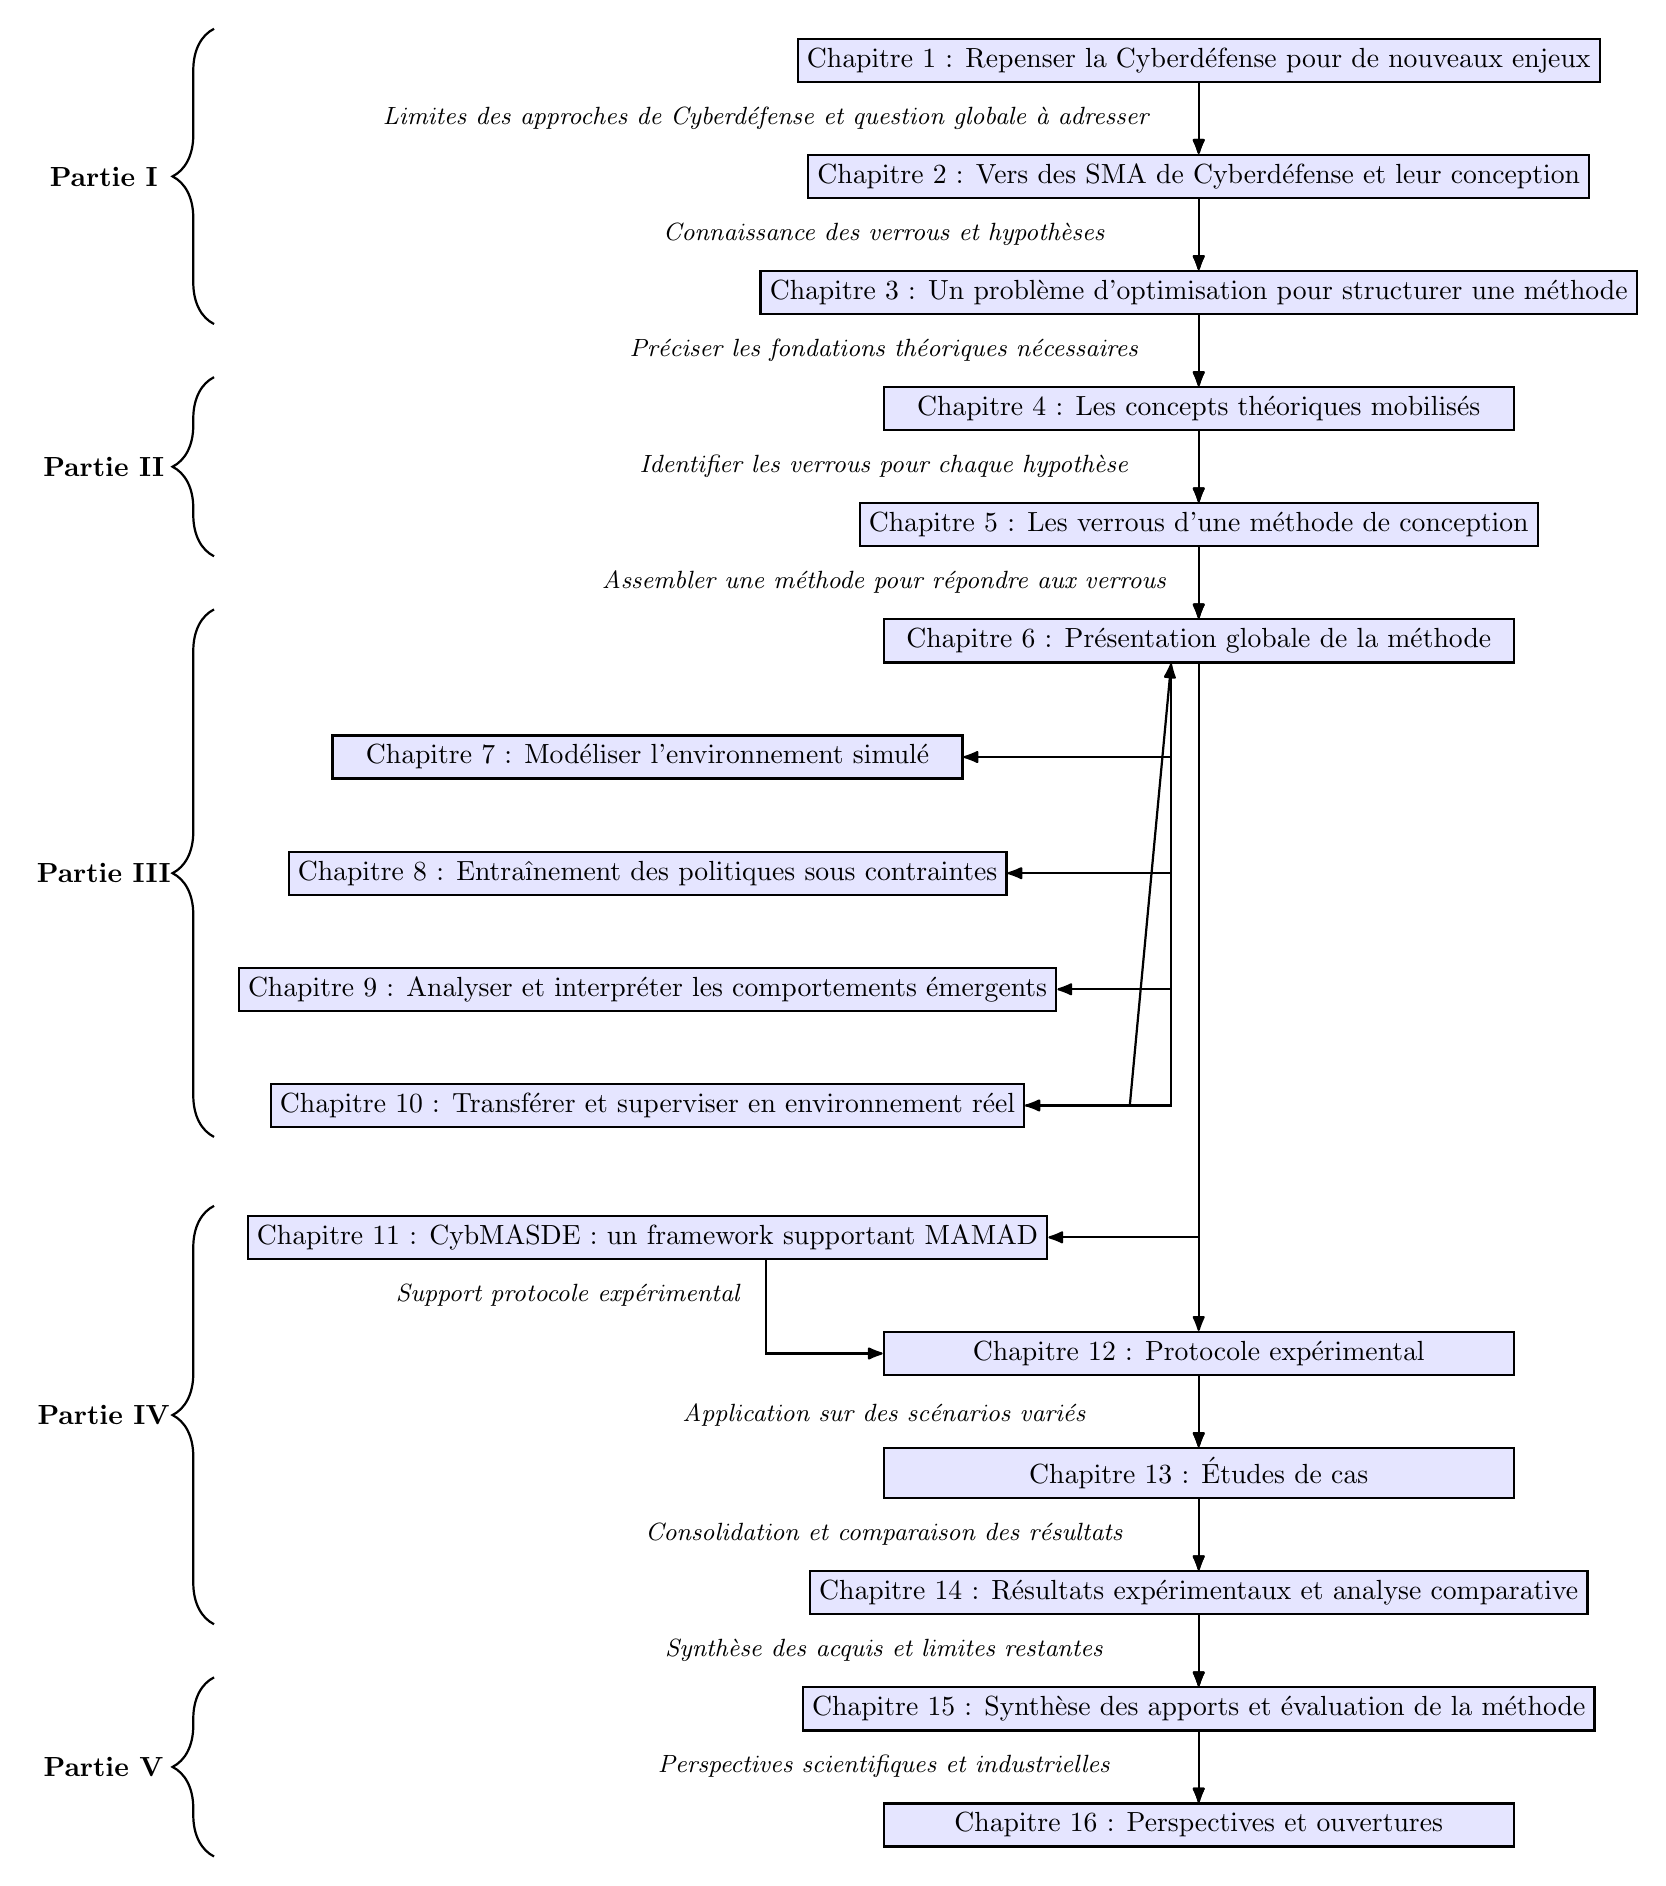
\begin{tikzpicture}[
    chapter/.style = {draw, thick, fill=blue!10, minimum width=8cm, align=left, font=\normalsize},
    arrow/.style = {-{Latex[round]}, thick},
    partlabel/.style = {rotate=90, font=\bfseries, align=center},
    dashedline/.style = {red, thick, dashed},
    node distance=0.9cm and 2cm,
    annotated/.style={above,font=\small\itshape, inner sep=1pt, yshift=5.5mm, xshift=-4cm}
    ]

    % Chapitres principaux (colonne verticale)
    \node[chapter] (c1) {Chapitre 1 : Repenser la Cyberdéfense pour de nouveaux enjeux};
    \node[chapter, below=of c1] (c2) {Chapitre 2 : Vers des SMA de Cyberdéfense et leur conception};
    \node[chapter, below=of c2] (c3) {Chapitre 3 : Un problème d'optimisation pour structurer une méthode};

    \node[chapter, below=of c3] (c4) {Chapitre 4 : Les concepts théoriques mobilisés};
    \node[chapter, below=of c4] (c5) {Chapitre 5 : Les verrous d'une méthode de conception};

    \node[chapter, below=of c5] (c6) {Chapitre 6 : Présentation globale de la méthode};

    % Flèches verticales principales avec annotations
    \draw[arrow] (c1) -- (c2) node[annotated, xshift=-1.5cm] {Limites des approches de Cyberdéfense et question globale à adresser};
    \draw[arrow] (c2) -- (c3) node[annotated] {Connaissance des verrous et hypothèses};
    \draw[arrow] (c3) -- (c4) node[annotated] {Préciser les fondations théoriques nécessaires};
    \draw[arrow] (c4) -- (c5) node[annotated] {Identifier les verrous pour chaque hypothèse};
    \draw[arrow] (c5) -- (c6) node[annotated] {Assembler une méthode pour répondre aux verrous};

    % Branche de droite (activités)
    \node[chapter, below= of c6, xshift=-7cm] (c7) {Chapitre 7 : Modéliser l'environnement simulé};
    \node[chapter, below=of c7] (c8) {Chapitre 8 : Entraînement des politiques sous contraintes};
    \node[chapter, below=of c8] (c9) {Chapitre 9 : Analyser et interpréter les comportements émergents};
    \node[chapter, below=of c9] (c10) {Chapitre 10 : Transférer et superviser en environnement réel};

    % Suite verticale
    \node[chapter, below=7cm of c6, xshift=-7cm] (c11) {Chapitre 11 : CybMASDE : un framework supportant MAMAD};
    \node[chapter, below=of c11, xshift=7cm] (c12) {Chapitre 12 : Protocole expérimental};
    \node[chapter, below=of c12] (c13) {Chapitre 13 : Études de cas};
    \node[chapter, below=of c13] (c14) {Chapitre 14 : Résultats expérimentaux et analyse comparative};
    \node[chapter, below=of c14] (c15) {Chapitre 15 : Synthèse des apports et évaluation de la méthode};

    \node[chapter, below=of c15] (c16) {Chapitre 16 : Perspectives et ouvertures};

    % Arrows
    \foreach \i/\j in {c1/c2, c2/c3, c3/c4, c4/c5, c5/c6, c12/c13, c13/c14, c14/c15, c15/c16}
    \draw[arrow] (\i) -- (\j);

    % Flèches horizontales depuis c6
    \foreach \dest in {c7, c8, c9, c10}
    \draw[arrow] ($ (c6.south) + (-0.35,0) $) -- ++(0,0) |- (\dest.east);

    \draw[arrow] (c10.east) -- ++(1.325,0) -- ($ (c6.south) + (-0.35,0) $);

    \draw[arrow] (c6.south) -- ++(0,0) |- (c11.east);

    \draw[arrow] ($ (c11.south) + (1.5, 0) $) -- ++(0,0) |- (c12.west) node[annotated] {Support protocole expérimental};

    \draw[arrow] (c6.south) -- (c12.north);


    % Flèches suite expérimentale
    \draw[arrow] (c12) -- (c13) node[annotated] {Application sur des scénarios variés};
    \draw[arrow] (c13) -- (c14) node[annotated] {Consolidation et comparaison des résultats};
    \draw[arrow] (c14) -- (c15) node[annotated] {Synthèse des acquis et limites restantes};
    \draw[arrow] (c15) -- (c16) node[annotated] {Perspectives scientifiques et industrielles};


    % Partie labels à gauche
    \draw[decorate, decoration={brace, amplitude=15pt}, thick]
    ($(c9.west |- c3.west)+(-0.3,-0.4)$) -- ($(c9.west |- c1.west)+(-0.3,0.4)$)
    node[midway,xshift=-1.4cm,rotate=0]{\textbf{Partie I}};

    \draw[decorate, decoration={brace, amplitude=15pt}, thick]
    ($(c9.west |- c5.west)+(-0.3,-0.4)$) -- ($(c9.west |- c4.west)+(-0.3,0.4)$)
    node[midway,xshift=-1.4cm,rotate=0]{\textbf{Partie II}};

    \draw[decorate, decoration={brace, amplitude=15pt}, thick]
    ($(c9.west |- c10.west)+(-0.3,-0.4)$) -- ($(c9.west |- c6.west)+(-0.3,0.4)$)
    node[midway,xshift=-1.4cm,rotate=0]{\textbf{Partie III}};

    \draw[decorate, decoration={brace, amplitude=15pt}, thick]
    ($(c9.west |- c14.west)+(-0.3,-0.4)$) -- ($(c9.west |- c11.west)+(-0.3,0.4)$)
    node[midway,xshift=-1.4cm,rotate=0]{\textbf{Partie IV}};

    \draw[decorate, decoration={brace, amplitude=15pt}, thick]
    ($(c9.west |- c16.west)+(-0.3,-0.4)$) -- ($(c9.west |- c15.west)+(-0.3,0.4)$)
    node[midway,xshift=-1.4cm,rotate=0]{\textbf{Partie V}};

  \end{tikzpicture}
}

    }
    \caption{Schéma de l'organisation du manuscrit}
\end{figure}

% =================================================================

\part{Fondements théoriques, revue de littérature et verrous}

\begin{figure}[h!]
    \centering
    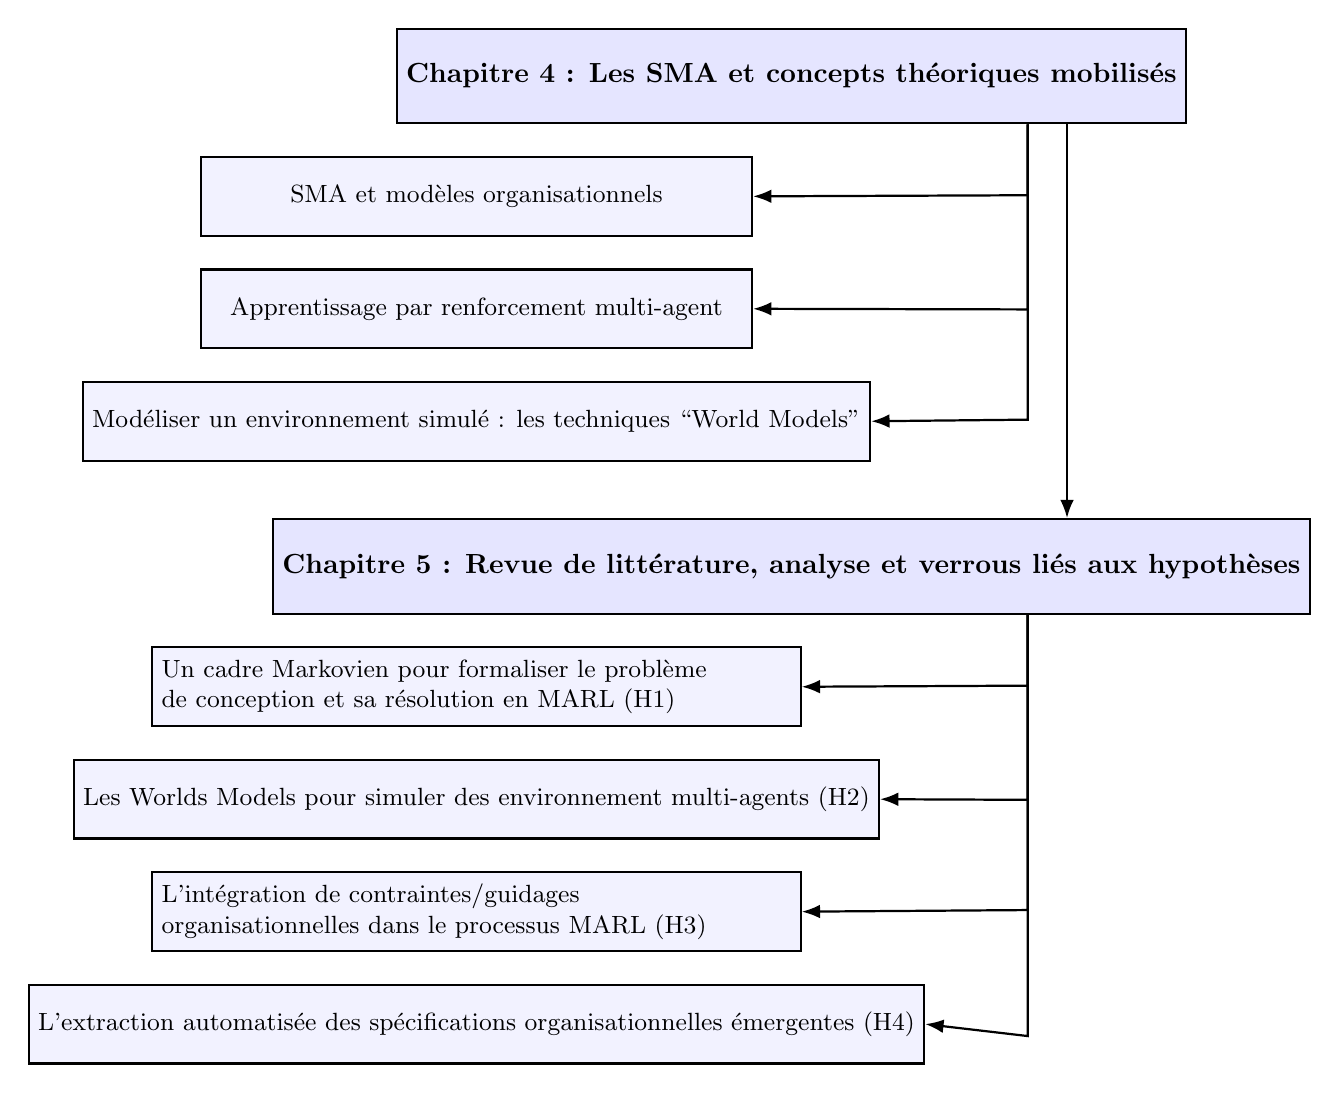
\begin{tikzpicture}[
    chapter/.style={draw, fill=blue!10, thick, minimum width=8cm, minimum height=1.2cm, text centered, font=\bfseries},
    section/.style={draw, fill=blue!5, thick, minimum width=7cm, minimum height=1cm, text centered, font=\small},
    arrow/.style={-Latex, thick},
    node distance=0.4cm
]

% Chapitre 4
\node[chapter] (ch4) {Chapitre 4 : Les SMA et concepts théoriques mobilisés};

\node[section, below=of ch4, xshift=-4cm] (ch4s1) {SMA et modèles organisationnels};
\node[section, below=of ch4s1] (ch4s2) {Apprentissage par renforcement multi-agent};
\node[section, below=of ch4s2] (ch4s3) {Modéliser un environnement simulé : les techniques \textquote{World Models}};

\draw[arrow] ($ (ch4.south) + (3,0) $) -- ++(0.,-0.9) -- (ch4s1.east);
\draw[arrow] ($ (ch4.south) + (3,0) $) -- ++(0.,-2.35) -- (ch4s2.east);
\draw[arrow] ($ (ch4.south) + (3,0) $) -- ++(0.,-3.75) -- (ch4s3.east);

% Chapitre 5
\node[chapter, below=5cm of ch4] (ch5) {Chapitre 5 : Revue de littérature, analyse et verrous liés aux hypothèses};

\node[section, below=of ch5, xshift=-4cm] (ch5s1) {\parbox{8cm}{Un cadre Markovien pour formaliser le problème \\ de conception et sa résolution en MARL (H1)}};
\node[section, below=of ch5s1] (ch5s2) {Les Worlds Models pour simuler des environnement multi-agents (H2)};
\node[section, below=of ch5s2] (ch5s3) {\parbox{8cm}{L'intégration de contraintes/guidages \\ organisationnelles dans le processus MARL (H3)}};
\node[section, below=of ch5s3] (ch5s4) {L'extraction automatisée des spécifications organisationnelles émergentes (H4)};

\draw[arrow] ($ (ch4.south) + (3.5,0) $) -- ($ (ch5.north) + (3.5,0) $);

\draw[arrow] ($ (ch5.south) + (3,0) $) -- ++(0.,-0.9) -- (ch5s1.east);
\draw[arrow] ($ (ch5.south) + (3,0) $) -- ++(0.,-2.35) -- (ch5s2.east);
\draw[arrow] ($ (ch5.south) + (3,0) $) -- ++(0.,-3.75) -- (ch5s3.east);
\draw[arrow] ($ (ch5.south) + (3,0) $) -- ++(0.,-5.35) -- (ch5s4.east);

\end{tikzpicture}

    \caption{Structure de la Partie II — Fondements théoriques, revue de littérature et verrous}
\end{figure}

\chapter{Concepts transversaux liés aux hypothèses}
% Objectif : définir les notions et modèles fondamentaux communs aux contributions.

\section{Systèmes Multi-Agents : coordination, rôles, interactions}
\section{Modèles organisationnels : MOISE+}

\section{Apprentissage par renforcement multi-agent (MARL)}

\section{Techniques \textquote{World Models}}

\chapter{Revue de littérature, analyse et verrous liés aux hypothèses}
% Objectif : pour chaque hypothèse H1–H5, analyser le domaine lié, identifier un manque, et formuler l'hypothèse comme réponse.

\section{H1 : Formalisation du problème (Dec-POMDP contraint)}
\section{H2 : Modélisation par apprentissage de l'environnement (World Models)}
\section{H3 : Résolution par MARL adaptatif}
\section{H4 : Guidage organisationnel via contraintes MOISE+ (OAC/TRF)}
\section{H5 : Analyse organisationnelle (rôles/objectifs émergents)}

\part{Méthode de conception : MAMAD}

\begin{figure}[h!]
    \centering
    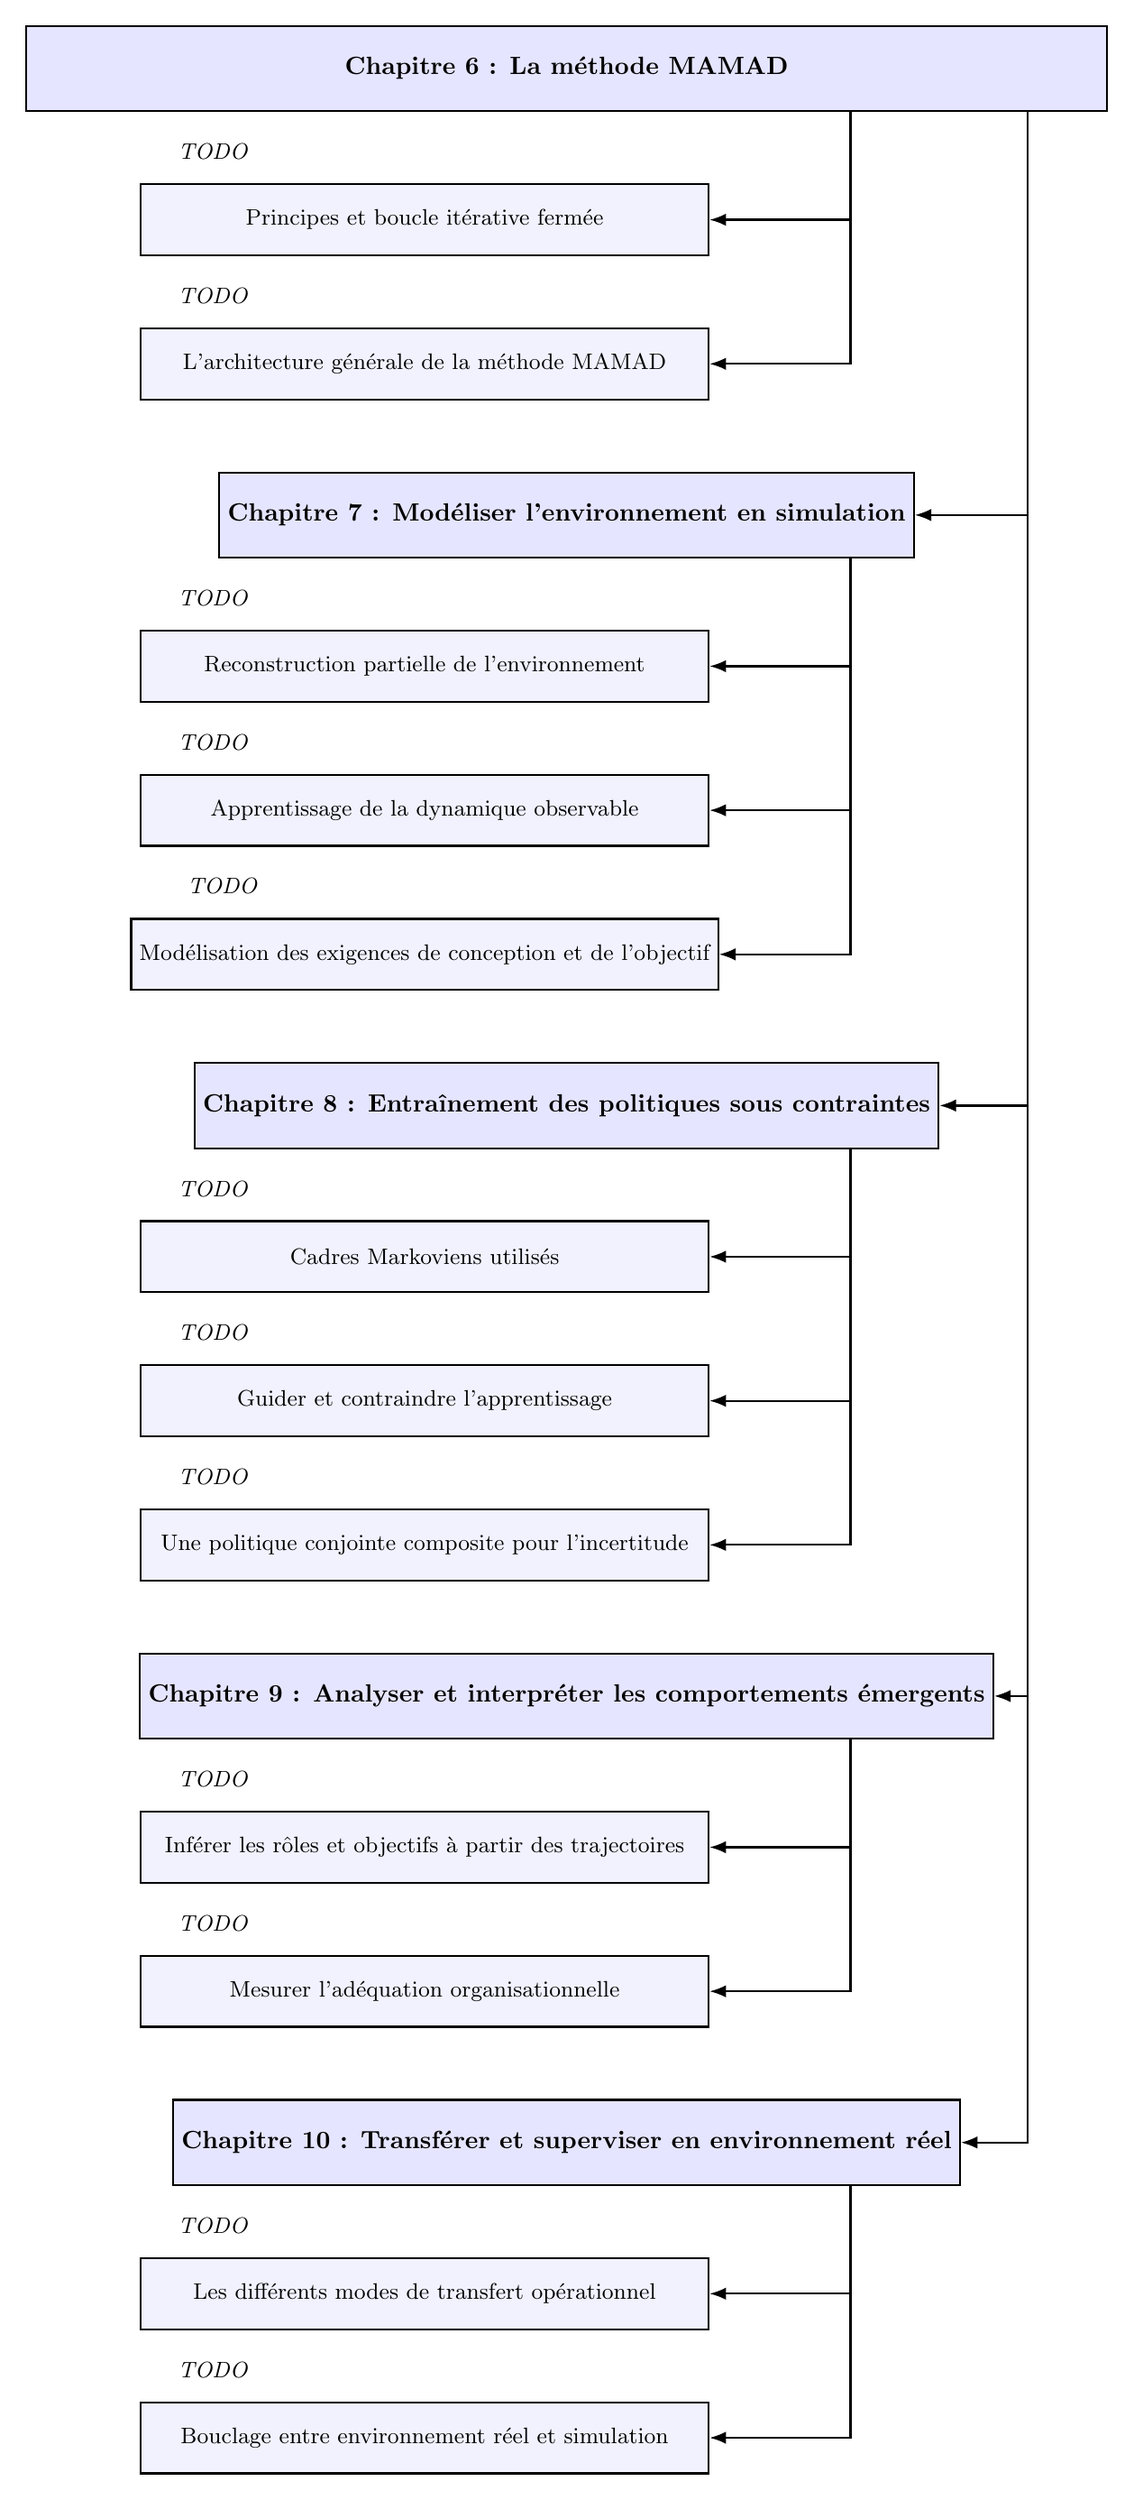
\begin{tikzpicture}[
    chapter/.style={draw, fill=blue!10, thick, minimum width=9cm, minimum height=1.2cm, text centered, font=\bfseries},
    section/.style={draw, fill=blue!5, thick, minimum width=8cm, minimum height=1cm, text centered, font=\small},
    arrow/.style={-Latex, thick},
    node distance=0.4cm,
    annotated/.style={above,font=\small\itshape, inner sep=1pt, yshift=0.8cm, xshift=-7cm}
]

% Chapitre 6 : MAMAD comme réponse
\node[chapter] (ch6) {\parbox{15cm}{\centering Chapitre 6 : La méthode MAMAD}};
\node[section, below=1cm of ch6, xshift=-2cm] (ch6s1) {Principes et boucle itérative fermée};
\node[section, below=1cm of ch6s1] (ch6s2) {L'architecture générale de la méthode MAMAD};

\draw[arrow] ($ (ch6.south) + (4.0,0) $) -- ++(0,0) |- (ch6s1.east) node[annotated] {TODO};
\draw[arrow] ($ (ch6.south) + (4.0,0) $) -- ++(0,0) |- (ch6s2.east) node[annotated] {TODO};

% Chapitre 7 : Phase 1 — Modélisation
\node[chapter, below=1cm of ch6s2, xshift=2cm] (ch7) {Chapitre 7 : Modéliser l'environnement en simulation};
\node[section, below=1cm of ch7, xshift=-2cm] (ch7s1) {Reconstruction partielle de l’environnement};
\node[section, below=1cm of ch7s1] (ch7s2) {Apprentissage de la dynamique observable};
\node[section, below=1cm of ch7s2] (ch7s3) {Modélisation des exigences de conception et de l'objectif};

\draw[arrow] ($ (ch7.south) + (4.0,0) $) -- ++(0,0) |- (ch7s1.east) node[annotated] {TODO};
\draw[arrow] ($ (ch7.south) + (4.0,0) $) -- ++(0,0) |- (ch7s2.east) node[annotated] {TODO};
\draw[arrow] ($ (ch7.south) + (4.0,0) $) -- ++(0,0) |- (ch7s3.east) node[annotated] {TODO};

% Chapitre 8 : Phase 2 — Apprentissage guidé
\node[chapter, below=1cm of ch7s3, xshift=2cm] (ch8) {Chapitre 8 : Entraînement des politiques sous contraintes};
\node[section, below=1cm of ch8, xshift=-2cm] (ch8s1) {Cadres Markoviens utilisés};
\node[section, below=1cm of ch8s1] (ch8s2) {Guider et contraindre l'apprentissage};
\node[section, below=1cm of ch8s2] (ch8s3) {Une politique conjointe composite pour l'incertitude};

\draw[arrow] ($ (ch8.south) + (4.0,0) $) -- ++(0,0) |- (ch8s1.east) node[annotated] {TODO};
\draw[arrow] ($ (ch8.south) + (4.0,0) $) -- ++(0,0) |- (ch8s2.east) node[annotated] {TODO};
\draw[arrow] ($ (ch8.south) + (4.0,0) $) -- ++(0,0) |- (ch8s3.east) node[annotated] {TODO};

% Chapitre 9 : Phase 3 — Analyse
\node[chapter, below=1cm of ch8s3, xshift=2cm] (ch9) {Chapitre 9 : Analyser et interpréter les comportements émergents};
\node[section, below=1cm of ch9, xshift=-2cm] (ch9s1) {Inférer les rôles et objectifs à partir des trajectoires};
\node[section, below=1cm of ch9s1] (ch9s2) {Mesurer l’adéquation organisationnelle};

\draw[arrow] ($ (ch9.south) + (4.0,0) $) -- ++(0,0) |- (ch9s1.east) node[annotated] {TODO};
\draw[arrow] ($ (ch9.south) + (4.0,0) $) -- ++(0,0) |- (ch9s2.east) node[annotated] {TODO};


% Chapitre 10 : Phase 4 — Transfert
\node[chapter, below=1cm of ch9s2, xshift=2cm] (ch10) {Chapitre 10 : Transférer et superviser en environnement réel};
\node[section, below=1cm of ch10, xshift=-2cm] (ch10s1) {Les différents modes de transfert opérationnel};
\node[section, below=1cm of ch10s1] (ch10s2) {Bouclage entre environnement réel et simulation};

\draw[arrow] ($ (ch10.south) + (4.0,0) $) -- ++(0,0) |- (ch10s1.east) node[annotated] {TODO};
\draw[arrow] ($ (ch10.south) + (4.0,0) $) -- ++(0,0) |- (ch10s2.east) node[annotated] {TODO};


\draw[arrow] ($ (ch6.south) + (6.5,0) $) -- ++(0,0) |- (ch7.east);
\draw[arrow] ($ (ch6.south) + (6.5,0) $) -- ++(0,0) |- (ch8.east);
\draw[arrow] ($ (ch6.south) + (6.5,0) $) -- ++(0,0) |- (ch9.east);
\draw[arrow] ($ (ch6.south) + (6.5,0) $) -- ++(0,0) |- (ch10.east);


\end{tikzpicture}

    \caption{Structure de la Partie III — Méthode de conception : MAMAD}
\end{figure}

\chapter{MAMAD comme réponse}

\section{Principe général et boucle itérative}

\section{Architecture globale}

\chapter{Phase 1 — Modélisation en simulation}
\section{Reconstruction partielle de l'environnement}
\section{Apprentissage de la dynamique observable}
\section{Intégration des contraintes de déploiement}

\chapter{Phase 2 — Apprentissage guidé/contraint}
\section{Cadres d'entraînement MARL utilisés}
\section{Contraintes organisationnelles dans MARL (OAC, TRF)}
\section{Politique composite et filtrage d'actions}

\chapter{Phase 3 — Analyse post-entraînement}
\section{Méthodes d'inférence des rôles et objectifs}
\section{Indicateurs : SOF, FOF, OF}
\section{Outil TEMM : fonctionnement, cas d'usage}

\chapter{Phase 4 — Transfert et supervision}
\section{Modes de transfert (centralisé/distribué)}
\section{Bouclage entre environnement réel et simulation}

\part{Cadre expérimental et analyse des résultats}

\begin{figure}[h!]
    \centering
    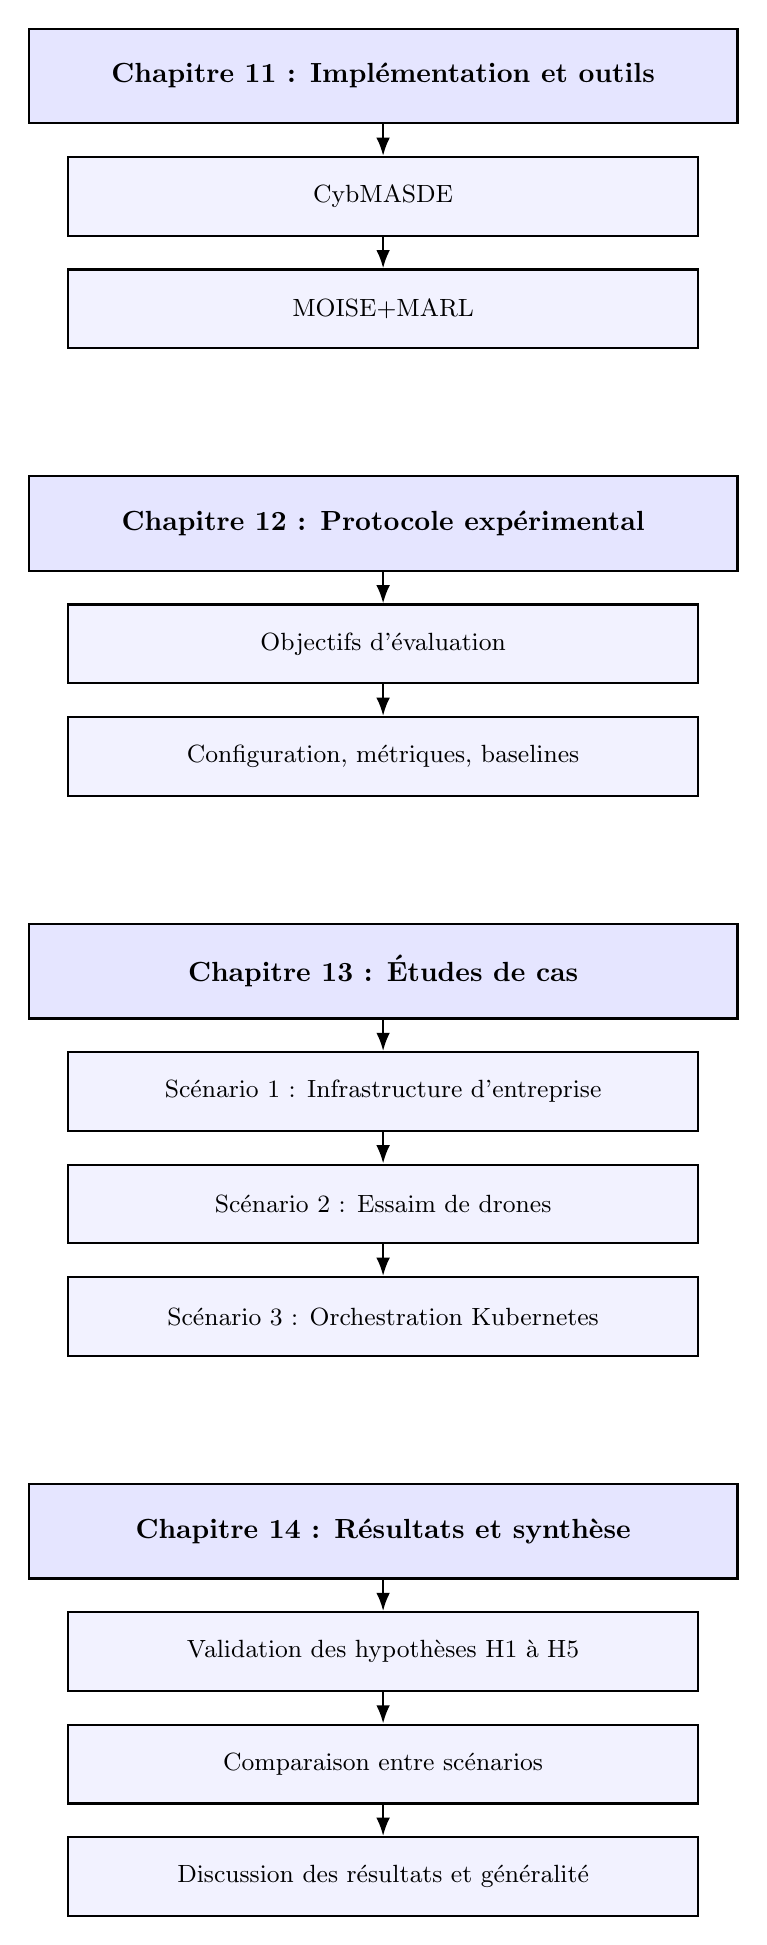
\begin{tikzpicture}[
    chapter/.style={draw, fill=blue!10, thick, minimum width=9cm, minimum height=1.2cm, text centered, font=\bfseries},
    section/.style={draw, fill=blue!5, thick, minimum width=8cm, minimum height=1cm, text centered, font=\small},
    arrow/.style={-Latex, thick},
    node distance=0.4cm
]

% Chapitre 11 : Implémentation et outils
\node[chapter] (ch11) {Chapitre 11 : Implémentation et outils};
\node[section, below=of ch11] (ch11s1) {CybMASDE};
\node[section, below=of ch11s1] (ch11s2) {MOISE+MARL};

\draw[arrow] (ch11) -- (ch11s1);
\draw[arrow] (ch11s1) -- (ch11s2);

% Chapitre 12 : Protocole expérimental
\node[chapter, below=1.6cm of ch11s2] (ch12) {Chapitre 12 : Protocole expérimental};
\node[section, below=of ch12] (ch12s1) {Objectifs d’évaluation};
\node[section, below=of ch12s1] (ch12s2) {Configuration, métriques, baselines};

\draw[arrow] (ch12) -- (ch12s1);
\draw[arrow] (ch12s1) -- (ch12s2);

% Chapitre 13 : Études de cas
\node[chapter, below=1.6cm of ch12s2] (ch13) {Chapitre 13 : Études de cas};
\node[section, below=of ch13] (ch13s1) {Scénario 1 : Infrastructure d’entreprise};
\node[section, below=of ch13s1] (ch13s2) {Scénario 2 : Essaim de drones};
\node[section, below=of ch13s2] (ch13s3) {Scénario 3 : Orchestration Kubernetes};

\draw[arrow] (ch13) -- (ch13s1);
\draw[arrow] (ch13s1) -- (ch13s2);
\draw[arrow] (ch13s2) -- (ch13s3);

% Chapitre 14 : Résultats et synthèse
\node[chapter, below=1.6cm of ch13s3] (ch14) {Chapitre 14 : Résultats et synthèse};
\node[section, below=of ch14] (ch14s1) {Validation des hypothèses H1 à H5};
\node[section, below=of ch14s1] (ch14s2) {Comparaison entre scénarios};
\node[section, below=of ch14s2] (ch14s3) {Discussion des résultats et généralité};

\draw[arrow] (ch14) -- (ch14s1);
\draw[arrow] (ch14s1) -- (ch14s2);
\draw[arrow] (ch14s2) -- (ch14s3);

\end{tikzpicture}

    \caption{Structure de la Partie IV — Cadre expérimental et analyse des résultats}
\end{figure}

\chapter{Implémentation et outils}
\section{CybMASDE}
\section{MOISE+MARL}

\chapter{Protocole expérimental}
\section{Objectifs d'évaluation}
\section{Configuration, métriques, baselines}

\chapter{Études de cas}
\section{Scénario 1 : Infrastructure d'entreprise}
\section{Scénario 2 : Essaim de drones}
\section{Scénario 3 : Orchestration Kubernetes}

\chapter{Résultats et synthèse}
\section{Validation des hypothèses H1 à H5}
\section{Comparaison entre scénarios}
\section{Discussion des résultats et généralité}

\part{Conclusion et perspectives}

\begin{figure}[h!]
    \centering
    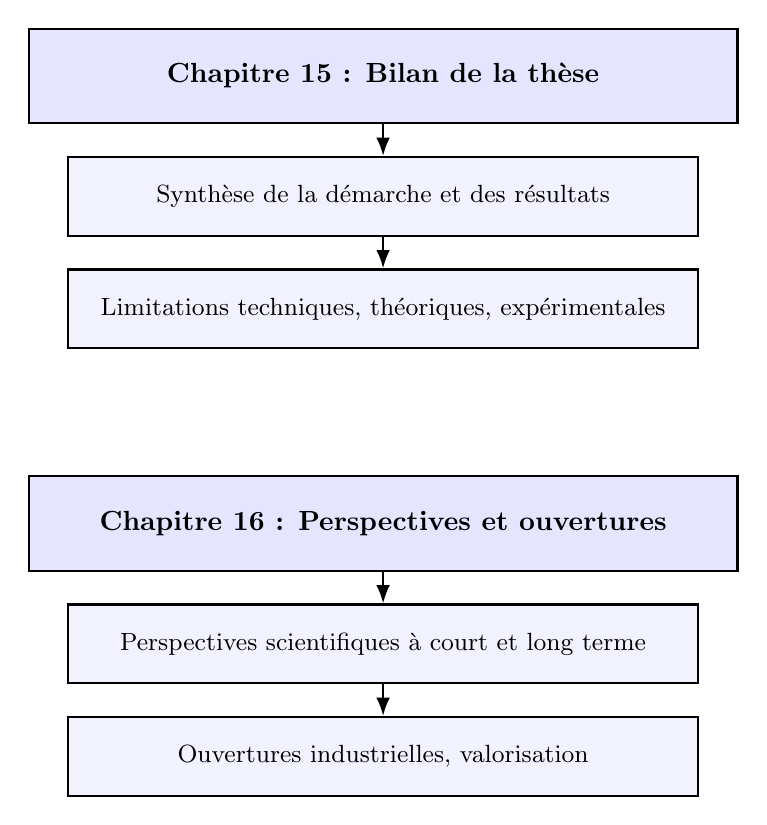
\begin{tikzpicture}[
    chapter/.style={draw, fill=blue!10, thick, minimum width=9cm, minimum height=1.2cm, text centered, font=\bfseries},
    section/.style={draw, fill=blue!5, thick, minimum width=8cm, minimum height=1cm, text centered, font=\small},
    arrow/.style={-Latex, thick},
    node distance=0.4cm
]

% Chapitre 15 : Bilan de la thèse
\node[chapter] (ch15) {Chapitre 15 : Bilan de la thèse};
\node[section, below=of ch15] (ch15s1) {Synthèse de la démarche et des résultats};
\node[section, below=of ch15s1] (ch15s2) {Limitations techniques, théoriques, expérimentales};

\draw[arrow] (ch15) -- (ch15s1);
\draw[arrow] (ch15s1) -- (ch15s2);

% Chapitre 16 : Perspectives et ouvertures
\node[chapter, below=1.6cm of ch15s2] (ch16) {Chapitre 16 : Perspectives et ouvertures};
\node[section, below=of ch16] (ch16s1) {Perspectives scientifiques à court et long terme};
\node[section, below=of ch16s1] (ch16s2) {Ouvertures industrielles, valorisation};

\draw[arrow] (ch16) -- (ch16s1);
\draw[arrow] (ch16s1) -- (ch16s2);

\end{tikzpicture}

    \caption{Structure de la Partie V — Conclusion et perspectives}
\end{figure}

\chapter{Bilan de la thèse}

\section{Synthèse de la démarche et des résultats}

\section{Limitations techniques, théoriques, expérimentales}

\chapter{Perspectives et ouvertures}
\section{Perspectives scientifiques à court et long terme}
\section{Ouvertures industrielles, valorisation}


%********************************************************************
% Other Stuff in the Back
%*******************************************************
\cleardoublepage\include{FrontBackmatter/Bibliography}
% \cleardoublepage\include{FrontBackmatter/Declaration}
% \cleardoublepage\include{FrontBackmatter/Colophon}

% ********************************************************************
% Backmatter
%*******************************************************
\appendix
%\renewcommand{\thechapter}{\alph{chapter}}
\cleardoublepage
% \part{Appendix}

%********************************************************************
% Appendix
%*******************************************************
% If problems with the headers: get headings in appendix etc. right
%\markboth{\spacedlowsmallcaps{Appendix}}{\spacedlowsmallcaps{Appendix}}
\chapter{Appendices}

\section{List of included papers}

\section{Experiments details}


\end{document}
% ********************************************************************
